%%%%%%%%%%%%%%%%%%%%%%%%%%%%%

%%%% ijcai19.tex

\typeout{IJCAI-19 Instructions for Authors}

% These are the instructions for authors for IJCAI-19.

\documentclass{article}
\pdfpagewidth=8.5in
\pdfpageheight=11in
% The file ijcai19.sty is NOT the same than previous years'
\usepackage{ijcai19}

% Use the postscript times font!
\usepackage{times}
\usepackage{soul}
\usepackage{url}
\usepackage[hidelinks]{hyperref}
\usepackage[utf8]{inputenc}
\usepackage[small]{caption}
\usepackage{graphicx}
\usepackage{amsmath}
\usepackage{booktabs}
\usepackage{algorithm}
\usepackage{algorithmic}

\usepackage{tikz}
\usepackage{textcomp}
\usepackage{comment} 
\usepackage{amssymb}
\usepackage{amsmath}
\usepackage{amsthm}
\usepackage{xspace}
\usepackage{todonotes}
\usepackage{url}
\usepackage{paralist}
% \usepackage{algpseudocode}
\usepackage{caption}
\usepackage{subcaption}
\usepackage{dsfont}
\usepackage{array,multirow}
\usepackage{ifthen}

\urlstyle{same}





%% the rest of your preamble here
\newcommand\blfootnote[1]{%
  \begingroup
  \renewcommand\thefootnote{}\footnote{#1}%
  \addtocounter{footnote}{-1}%
  \endgroup
}







\newcommand\eva[1]{\textcolor{pink}{Eva: #1}}
\newcommand\toptile[1]{top_{#1}}
\newcommand\bottomtile[1]{bot_{#1}}
\newcommand\lefttile[1]{lef_{#1}}
\newcommand\righttile[1]{rig_{#1}}
\newcommand{\coms}{\xspace\scalebox{0.5}{
\begin{tikzpicture}\draw[dash pattern=on 3pt off 3pt, line width = 1mm ] (0,0) -- (0.8,0); \node at (0,-0.08) {}; \end{tikzpicture}}\xspace}
\newcommand{\moves}{\rightarrow}
\newcommand{\colorellipse}{orange!20!white}
\newcommand{\addCommunicationB}[1]
{
	\node[above right = 0.5mm and 4mm of #1, inner sep=0mm] (nb2) {B};
	\draw[tobehere,communication] (#1) -- (nb2);
}

\newcommand\setnodes{V}
\newcommand\basenode{B}
\newcommand{\sourcenode}{s}
\newcommand{\targetnode}{t}
\newcommand\USTCONN{USTCONN}
\newcommand\UCONN{UCONN}
\newcommand{\myundirectedgraphbounded}{\mathfrak G}
\newcommand{\myundirectedgraph}{\mathfrak G'}

\newcommand\pb[2]{${#1}_{#2}$~}

\newcommand\pbReach[1]{\pb{Reachability}{#1}}
\newcommand\pbBReach[1]{\pb{bReachability}{#1}}
\newcommand\pbCoverage[1]{\pb{Coverage}{#1}}
\newcommand\pbBCoverage[1]{\pb{bCoverage}{#1}}

\newcommand{\idDir}{dir}	% identifier for directed topological graph
\newcommand{\idNC}{nc}		% identifier for neighbor-communicable topological graph
\newcommand{\idSM}{sm}		% identifier for sight-moveable topological graph
\newcommand{\idCC}{cc}		% identifier for complete-communication topological graph
\newcommand{\idUnd}{und}		% identifier for complete-communication topological graph

\newcommand{\pbReachDir}{\pbReach{\idDir}}
\newcommand{\pbBReachDir}{\pbBReach{\idDir}}
\newcommand{\pbCoverageDir}{\pbCoverage{\idDir}}
\newcommand{\pbBCoverageDir}{\pbBCoverage{\idDir}}

\newcommand{\pbReachNC}{\pbReach{\idNC}}
\newcommand{\pbBReachNC}{\pbBReach{\idNC}}
\newcommand{\pbCoverageNC}{\pbCoverage{\idNC}}
\newcommand{\pbBCoverageNC}{\pbBCoverage{\idNC}}

\newcommand{\pbReachSM}{\pbReach{\idSM}}
\newcommand{\pbBReachSM}{\pbBReach{\idSM}}
\newcommand{\pbCoverageSM}{\pbCoverage{\idSM}}
\newcommand{\pbBCoverageSM}{\pbBCoverage{\idSM}}

\newcommand{\pbReachCC}{\pbReach{\idCC}}
\newcommand{\pbBReachCC}{\pbBReach{\idCC}}
\newcommand{\pbCoverageCC}{\pbCoverage{\idCC}}
\newcommand{\pbBCoverageCC}{\pbBCoverage{\idCC}}

\newcommand{\pbReachUnd}{\pbReach{\idUnd}}
\newcommand{\pbBReachUnd}{\pbBReach{\idUnd}}
\newcommand{\pbCoverageUnd}{\pbCoverage{\idUnd}}
\newcommand{\pbBCoverageUnd}{\pbBCoverage{\idUnd}}

\newtheorem{theorem}{Theorem}
\newtheorem{fact}[theorem]{Fact}
\newtheorem{definition}[theorem]{Definition}
\newtheorem{proposition}[theorem]{Proposition}
%\newtheorem{proof}{Proof}
\newtheorem{lemma}[theorem]{Lemma}

\tikzstyle{copyofG} = [fill=gray!20!white, draw=none, rounded corners=8pt]
\tikzstyle{communication} = [dash pattern=on 1pt off 1pt] %[line cap=rect, dot diameter=1pt, dot spacing=2pt, dots] %[dash pattern=on 2pt off 2pt on \the\pgflinewidth off 2pt]
\tikzstyle{tobehere} = [color=blue!50!white]
\newcommand\set[1]{\{#1\}}
\newcommand\suchthat{\mid}
\newcommand{\nbdrones}{n}

\newcommand{\booleanvariablegeneric}{{x}}
\newcommand{\clausegeneric}{\mathsf{c}}

\newcommand{\ok}{\includegraphics[height=2mm]{check.png}}
\newcommand{\imgDrone}{\includegraphics[height=2mm]{drone_black.png}}

\usetikzlibrary{decorations.pathmorphing}
\usetikzlibrary{decorations.pathreplacing}
\usetikzlibrary{arrows}
\usetikzlibrary{positioning}

\makeatletter
\tikzset{
	dot diameter/.store in=\dot@diameter,
	dot diameter=3pt,
	dot spacing/.store in=\dot@spacing,
	dot spacing=10pt,
	dots/.style={
		line width=\dot@diameter,
		line cap=round,
		dash pattern=on 0pt off \dot@spacing
	}
}
\makeatother

%%% Local Variables:
%%% mode: latex
%%% TeX-master: "main"
%%% End:



\newif\iffull
% \fullfalse
\fulltrue

\newif\ifauthor
%\authorfalse
\authortrue

{\renewcommand{\baselinestretch}{0.99}

% the following package is optional:
%\usepackage{latexsym} 

% Following comment is from ijcai97-submit.tex:
% The preparation of these files was supported by Schlumberger Palo Alto
% Research, AT\&T Bell Laboratories, and Morgan Kaufmann Publishers.
% Shirley Jowell, of Morgan Kaufmann Publishers, and Peter F.
% Patel-Schneider, of AT\&T Bell Laboratories collaborated on their
% preparation.

% These instructions can be modified and used in other conferences as long
% as credit to the authors and supporting agencies is retained, this notice
% is not changed, and further modification or reuse is not restricted.
% Neither Shirley Jowell nor Peter F. Patel-Schneider can be listed as
% contacts for providing assistance without their prior permission.

% To use for other conferences, change references to files and the
% conference appropriate and use other authors, contacts, publishers, and
% organizations.
% Also change the deadline and address for returning papers and the length and
% page charge instructions.
% Put where the files are available in the appropriate places.

% \title{IJCAI--19 Formatting Instructions}

\title{Reachability and Coverage Planning for Connected Agents:
		\large
		\\
		Extended Version}
% put your title here!

% Single author syntax
% \author{
%     Sarit Kraus
%     \affiliations
%     Department of Computer Science, Bar-Ilan University, Israel \emails
%     pcchair@ijcai19.org
% }


% Multiple author syntax (remove the single-author syntax above and the \iffalse ... \fi here)
% Check the ijcai19-multiauthor.tex file for detailed instructions
% \iffalse
\ifauthor
\author{
Tristan Charrier$^1$
\and
Arthur Queffelec$^1$\and
Ocan Sankur$^2$\And
Fran\c{c}ois Schwarzentruber$^1$
\affiliations
Univ Rennes, CNRS, IRISA$^1$\\
Univ Rennes, Inria, CNRS, IRISA$^2$\\
\emails
firstname.lastname@irisa.fr$^1$,
ocan.sankur@inria.fr$^2$,
}
\else
\author{\# 4601
% Tristan Charrier$^1$
% \and
% Arthur Queffelec$^1$\and
% Ocan Sankur$^2$\And
% Fran\c{c}ois Schwarzentruber$^3$
% \affiliations
% $^1$IRISA\\
% $^2$INRIA\\
% $^3$ENS Rennes
% \emails
% \{first, second\}@irisa.fr,
% third@inria.fr,
% fourth@ens-rennes.fr
}
\fi

\begin{document}

\maketitle

\begin{abstract}
	Motivated by the increasing appeal of robots in information-gathering missions,
	we study multi-agent path planning problems in which the agents must remain
	interconnected. We model an area by a topological graph specifying the movement
	and the connectivity constraints of the agents. We study the theoretical
	complexity of the reachability and the coverage problems of a fleet of connected
	agents on various classes of topological graphs.
	We establish the complexity of these problems on known classes, and introduce a new class
        called \emph{sight-moveable graphs}
        which admit efficient algorithms.
	% We show that deciding the existence of a covering plan is PSPACE-complete.
	% Additionally, we show that this complexity holds in a reasonable subclass of
	% topological graphs called the neighbor-communicable topological graphs. We
	% identify a realistic but restrictive subclass, the class of sight-moveable
	% topological graphs, on which the reachability and the coverage problems are in
	% LOGSPACE. However, the corresponding optimization problems of the makespan of
	% such plans remain NP-complete on all classes of topological graphs defined in
	% this work, except the complete-communication case in which the bounded
	% reachability falls in LOGSPACE.
	% Motivated by the increasing appeal of robots in information-gathering missions,
	% we study an approach to multi-agent path planning in which the agents are
	% interconnected. We model an area by a topological graph specifying the movement
	% and the connectivity constraints of the agents. We study the theoretical
	% complexity of the reachability and the coverage problems of a fleet of connected
	% agents on topological graphs.
	
	% We show that deciding the existence of a covering plan is PSPACE-complete.
	% Additionally, we show that this complexity holds in a reasonable subclass of
	% topological graphs called the neighbor-communicable topological graphs. We
	% identify a realistic but restrictive subclass, the class of sight-moveable
	% topological graphs, on which the reachability and the coverage problems are in
	% LOGSPACE. However, the corresponding optimization problems of the makespan of
	% such plans remain NP-complete on all classes of topological graphs defined in
	% this work, except the complete-communication case in which the bounded
	% reachability falls in LOGSPACE.
\end{abstract}

%  \begin{document}

\section{Introduction}
\label{sec:intro}



\IEEEPARstart{T}{wo} %
main challenges in the deployment of large-scale swarms are the localization and coordination of vehicles.
Localization methods that rely on external infrastructure 
(e.g., GPS) 
are prone to systematic errors (e.g., multipath effect)
and may not always be available.
Coordination strategies that are centralized can deconflict motion plans to prevent collisions and gridlock, but introduce a single point of failure and are difficult to scale in swarm size due to communication bandwidth limitations.

This paper presents a unified formation flying pipeline for unmanned aerial vehicles (UAVs).
Our pipeline uses \textit{onboard} sensors for localization, which eliminate the need for external positioning systems, and \textit{distributed} techniques for coordination, which enable each vehicle to make decisions independently while communicating their state to a subset of the team.
For \textit{localization}, we use an off-the-shelf commercial visual inertial odometry (VIO) package \cite{VIO}
that fuses inertial measurement unit (IMU) and downward-facing monocular camera measurements to estimate changes in the vehicle pose.
\edit{For \textit{coordination}, we present distributed formation control and task assignment strategies that run onboard the vehicles, do not rely on a common reference frame, and use vehicle-to-vehicle communication.} 
Key features of our formation control strategy include scalability to a large number of vehicles and robustness to disturbances.
The latter is crucial for reaching the desired formations with sensing imperfections.
Our task assignment strategy uses an auction-based algorithm to guarantee conflict-free assignments.
This algorithm can deconflict vehicle gridlocks resulting from distributed collision avoidance (type 3 deadlock~\cite{Wang2017}) and is well-suited for vehicles with limited computational capability and low-bandwidth communication. 


\begin{figure}[t!]
	\begin{center}
		\includegraphics[trim =0mm 10mm 0mm 0mm, clip, width=\columnwidth]{Figs/slanted_plane.png}	
		\caption{
		Six multirotors in a slanted plane formation.
		Vehicles communicate with each other, make distributed decisions onboard, and use VIO for localization.}
		\label{fig:slantedplane}
	\end{center}
\end{figure}


\subsection{Contributions}

This research extends our previous work on UAV formations~\cite{Fathian2019} and presents a unified pipeline consisting of \textit{onboard localization} and \textit{distributed coordination}.
The three main contributions of this work are:
\begin{enumerate}
    \item \edit{scalable formulation of control design suitable for
    onboard sensing without a common reference frame;}
    \item algorithms for deconfliction via \edit{distributed} task assignment of vehicles to desired formation points;    
    \item simulation- and hardware-ready open-source pipeline.
\end{enumerate}
\edit{Our pipeline is tested in hardware with six multirotors (see Fig.~\ref{fig:slantedplane}), and 
to our knowledge is the first demonstration of formation flying that does not rely on external sensing, fiducial markers for localization, a common reference frame, or a centralized base station for coordination.}
The only requirements for the presented pipeline are that the vehicles can communicate, can find the transformation between their VIO start frames, and the environment is sufficiently textured---a standard assumption for VIO systems.
As such, this framework paves the way for future, real-world deployments of aerial vehicle swarms in large numbers and without requiring external localization infrastructure.


\begin{figure} [t!]
\centering
	\begin{subfigure}[b]{0.32\columnwidth}
	   %
	    \includegraphics[width=0.8\textwidth,left]{Figs/Frames2_full.pdf}
	    \caption{\scriptsize full alignment}
	    \label{fig:frame-a}
	\end{subfigure}
	\begin{subfigure}[b]{0.32\columnwidth}
	    \includegraphics[width=0.8\textwidth,center]{Figs/Frames2_orientation.pdf}
	    \caption{\scriptsize orientation alignment}
	    \label{fig:frame-b}
	\end{subfigure}
	\begin{subfigure}[b]{0.32\columnwidth}
	    \includegraphics[width=0.8\textwidth,right]{Figs/Frames2_none.pdf}
	    \caption{\scriptsize no alignment}
        \label{fig:frame-c}
	\end{subfigure}
\caption{\edit{Required alignment of UAV frames in existing swarm strategies: (a) the most restrictive case requiring a common reference frame, i.e., orientation and origin of the frames must be aligned; (b) only the orientation of the frames must be aligned; (c) no alignment restrictions (this work).}}
	\label{fig:Frames}
\end{figure}




\subsection{Related Work}

Existing aerial swarms can be grouped based on the coordination (centralized vs.\ distributed) and localization (external vs.\ onboard) methods used. 
\edit{It is further crucial to distinguish these methods based on the level of alignment required for the vehicle coordinate frames; see Fig.~\ref{fig:Frames}.} 
 
\edit{
Works with \textit{centralized} coordination and \textit{external} localization include~\cite{Preiss2017, Honig2018, Du2019}, which are based on lightweight UAVs with limited onboard computational capability and therefore rely on an external motion capture system and a base station.
Works with \textit{distributed} coordination and \textit{external} localization include \cite{wilson2020robotarium}, \cite{enright2004spheres}, where robots execute distributed controls  based on external localization by motion capture and ultrasonic beacons, respectively.
Works with \textit{centralized} coordination and \textit{onboard} localization include~\cite{Forster2013}, \cite{Loianno2016}, which use a ground station for task assignment among vehicles.
In \cite{Weinstein2018}, formation flying based on VIO is demonstrated, where motion planning and assignment are run on a base station to ensure collision-free trajectories.
The coordination strategies used in aforementioned works require a \textit{common reference frame} (Fig.~\ref{fig:frame-a}).
}


\edit{
Despite the large body of work on formation control~\cite{Oh2015}, and the variety of onboard sensing solutions for localization (e.g., VIO~\cite{Delmerico2018}), few frameworks demonstrated formation flying with \textit{distributed} coordination and \textit{onboard} localization.
A key reason is reliance of many distributed control and assignment algorithms on aligned frames (Fig.~\ref{fig:frame-a}, \ref{fig:frame-b}), which require computation-expensive and/or communication-intensive synchronization/consensus steps for frame alignment.
Equally important, dependence on alignment in existing methods \cite{Wang2017,Turpin2014, van2011reciprocal, morgan2016swarm} diminishes robustness to inherent noise and unobservable errors that cannot be corrected (e.g., disparities between the actual and estimated body frame \textit{orientation} caused by VIO drift).
Leveraging coordination methods that are \textit{robust to misaligned frames} is hence crucial and a focus of this work. 
}






\edit{
Examples of other pipelines with distributed coordination and onboard localization include \cite{Montijano2016,Tron2016}.
Both works demonstrated formation flying on three UAVs, required information from an external motion capture system due to hardware limitations, did not incorporate collision avoidance, and required frame alignment.
}
\edittwo{Note that while~\cite{Montijano2016,Tron2016} can achieve formations with arbitrary headings as illustrated in Fig.~\ref{fig:frame-c}, knowledge of relative orientations is still required; therefore, they belong to the category of Fig.~\ref{fig:frame-b}.}






\if 0

\r{
decentralized coordination setting combined with VIO:
D-CAPT [26]~\cite{}:
ORCA ~\cite{}: 
CBF [2]~\cite{} :
[A]
}

\r{Robusteness in coordination,  with compounded noise/latency, which would eventually break (b).\\


some existing algorithm might as well
work in a similar fully decentralized setting, when combined with VIO
as proposed here. For example, D-CAPT [26], ORCA, CBF [2] might also be
useful for such a task and are computationally even more efficient than
the proposed approach. \\

R2:  onboard sensing for localization ->
 Finally, the related work section only
focuses on this aspect of the pipeline, discussing how many formation papers include
onboard localization but barely sells the advantages of the coordination module (the actual
proposal of the paper) against other competitors such as [26] or [A] or to mention similar
coordination pipelines. \\


Given a solution to this problem, the controller in Section III seems unnecessary, each drone
has a target position and can use a local controller with collision avoidance that drives it to
that position. Note that such controllers exists in the literature (e.g., RVO in any of its
multi-agent variantes), they are distributed in nature and only require local sensing.


}

\fi

\section{Preliminaries}
\label{sec:preli}

%In this section, we define the required notions used throughout the work.


%\subsection{Proof Overview} 

\section{Preliminaries}
\label{sec:prelims}
In the interest of getting quickly to the overview in \cref{sec:overview}, on a first pass reading of this paper, the reader may wish to skip over the (short) proofs later in this section.

\subsection{Algorithm}
%First, we recall the classical Christofides-Serdyukov algorithm: Given an instance of TSP, choose a minimum spanning tree and then add the minimum cost matching on the odd degree vertices of the tree. The algorithm we study is very similar, except we choose a random spanning tree based on the standard linear programming relaxation of TSP. 

Let $x^0$ be an optimum solution of LP \eqref{eq:tsplp}. 
%Without loss of generality, we assume that there is 
%It can be shown that $x^*$ always has an edge with fraction 1 \cite{BP90}).
Without loss of generality we assume $x^0$ has an edge $e_0=\{u_0,v_0\}$ with $x^0_{e_0}=1, c(e_0)=0$.
(To justify this, consider the following process: given $x^0$, pick an arbitrary node, $u$, split it into two nodes $u_0,v_0$ and set $x_{\{u_0,v_0\}}=1, c(e_0)=0$ and assign half of every edge incident to $u$ to $u_0$ and the other half to $v_0$.) %This allows us to assume without loss of generality that $x^0$ has an edge $e_0=(u_0,v_0)$ such that  $x_{e_0}=1, c(e_0)=0$. 

Let $E_0=E\cup\{e_0\}$ be the support of $x^0$ and let $x$ be $x^0$ restricted to $E$ and $G=(V,E)$. Note $x^0$ restricted to $E$ is in the spanning tree polytope  \eqref{eq:spanningtreelp} of $G$.

For a vector $\lambda:E\to\R_{\geq 0}$, a $\lambda$-uniform distribution $\mu_\lambda$ over spanning trees of $G=(V,E)$ is a distribution where for every spanning tree $T\subseteq E$, $\PP{\mu_\lambda}{T}=\frac{\prod_{e\in T} \lambda_e}{\sum_{T'} \prod_{e\in T'} \lambda_e}$.
The second step of the algorithm is to find a vector $\lambda$ such that for every edge $e\in E$, $\PP{T \sim \mu_\lambda}{e\in T}=x_e(1\pm\eps)$, for some $\eps<2^{-n}$. Such a vector $\lambda$ can be found using the multiplicative weight update algorithm \cite{AGMOS10} (see \cref{thm:maxentropycomp}) or by applying interior point methods \cite{SV12} or the ellipsoid method \cite{AGMOS10}. (We note that the multiplicative weight update method can only guarantee $\eps<1/\text{poly}(n)$ in polynomial time.)

Finally, similar to Christofides' algorithm, we sample a tree $T\sim\mu_{\lambda}$ and then add the minimum cost matching on the odd degree vertices of $T$.

\hypertarget{tar:alg}{\begin{algorithm}[h]
\begin{algorithmic}
	\State Find an optimum solution $x^0$ of  \cref{eq:tsplp}, and let $e_0=\{u_0,v_0\}$ be an edge with $x^0_{e_0}=1,c(e_0)=0$.
	\State Let $E_0=E\cup \{e_0\}$ be the support of $x^0$ and $x$ be $x^0$ restricted to $E$ and $G=(V,E)$.
	\State Find a vector $\lambda:E\to\R_{\geq 0}$ such that for any $e\in E$, $\PP{T \sim \mu_\lambda}{e \in T}=x_e(1\pm 2^{-n})$.
	\State Sample a tree $T\sim\mu_\lambda$.
	\State Let $M$ be the minimum cost matching on odd degree vertices of $T$.
	\State Output $T \cup M$.
\end{algorithmic}
\caption{Max Entropy Algorithm for TSP}\label{alg:tsp}
\end{algorithm}}
The above algorithm from \cite{KKO21} is a slight modification of the algorithm proposed in  \cite{OSS11}. While the proof of \cref{thm:main} heavily utilizes properties of max entropy trees, we note that \cref{thm:cutsbothsideswithinside} (the main contribution of this paper) only uses the fact that the spanning tree distribution respects the marginals of $x$.
\begin{theorem}[\cite{AGMOS10}]
\label{thm:maxentropycomp}
Let $z$ be a point in the spanning tree polytope (see \eqref{eq:spanningtreelp}) of a graph $ G=(V, E)$.
For any $\eps>0$, a vector $\lambda:E\to\R_{\geq 0}$ can be found such that the corresponding $\lambda$-uniform spanning tree distribution, $\mu_\lambda$, satisfies
%we define the exponential family distribution
%$$\tilde{p}(T):=\frac{1}{P}\exp(\sum_{e\in T} \tilde{\gamma}_e)$$ for
%all $T\in {\cal T}$ where $$P:=\sum_{T\in {\cal T}}\exp(\sum_{e\in T}
%\tilde{\gamma}_e)$$ then, for every edge $e\in E$,
$$%\tilde{z}_e :=
\sum_{T\in {\cal T}: T \ni e} \PP{\mu_\lambda}{T}  \leq (1+\varepsilon)z_e,\hspace{3ex}\forall e\in E,$$
i.e., the marginals are approximately preserved.  In the above ${\cal T}$ is the set of all spanning trees of $(V,E)$. The running
time is polynomial in $n=|V|$, $- \log \min_{e\in E} z_e$ and $\log(1/\eps)$.
\end{theorem}

%\subsection{Held-Karp relaxation and class of algorithms}
%
%Let $x^0$ be an optimum solution of the following TSP   linear program relaxation \cite{DFJ59,HK70}:
%\begin{equation}\label{eq:tsplp}
%\begin{aligned}
%	\min \quad& \sum_{u,v} x_{(u,v)} c(u,v)& \\
%	\text{s.t.,} \quad &  \sum_{u} x_{(u,v)} = 2&\forall v\in V,\\
%	& \sum_{u\in S, v\notin S} x_{(u,v)}\geq 2,&\forall S\subsetneq V,\\
%	& x_{(u,v)}\geq 0 &\forall u,v\in V.
%\end{aligned}	
%\end{equation}
%
%Given  $x^0$, we pick an arbitrary node, $u$, split it into two nodes $u_0,v_0$ and set $x_{(u_0,v_0)}=1, c(u_0,v_0)=0$ and we assign half of every edge incident to $u$ to $u_0$ and the other half to $v_0$.  This allows us to assume without loss of generality that $x^0$ has an edge $e_0=(u_0,v_0)$  such that  $x_{e_0}=1, c(e_0)=0$. 
%%if such an edge does not exist, we (also 
%
%Let $E_0=E\cup\{e_0\}$ be the support of $x^0$ and let $x$ be $x^0$ restricted to $E$ and $G=(V,E)$.
%% be the support of $x$ excluding the edge $e_0$, and let $E_0=E\cup \{e_0\}$.
%$x^0$ restricted to $E$ is in the spanning tree polytope. The algorithm samples a tree from $x^0$ and then adds the edge $e_0$. 

\subsection{Notation}
We write $[n]:=\{1,\dots,n\}$ to denote the set of integers from $1$ to $n$.
For a set of edges $A\subseteq E$ and (a tree) $T\subseteq E$, we write\footnote{We put this notation in a box because it is so important and ubiquitous in this paper.} 
$$\boxed{\hypertarget{tar:AT}{A_T = |A \cap T|}.}$$
For a set $S\subseteq V$, we write 
$$E(S)=\{\{u,v\}\in E: u,v\in S\}$$ to denote the set of edges in $S$ and we write 
$$\delta(S)=\{\{u,v\}\in E: |\{u,v\}\cap S|=1\}$$ 
to denote the  set of edges that leave $S$. 
For two {\em disjoint} sets of vertices $A,B\subseteq V$, we write
$$ E(A,B)=\{\{u,v\}\in E: u\in A, v\in B\}.$$
For a set $A\subseteq E$ and a function $x:E\to\R$ we write
$$ x(A):=\sum_{e\in A} x_e.$$
\hypertarget{tar:crossing}{For two sets $A,B\subseteq V$, we say $A$ {\em crosses} $B$ if all of the following sets are non-empty:
$$ A\cap B, A\smallsetminus B, B\smallsetminus A, \overline{A\cup B}.$$}
\hypertarget{tar:G=(V,E,x)}{We write $G=(V,E,x)$ to denote an (undirected) graph $G$ together with special vertices $u_0,v_0$ and a weight function $x:E\to\R_{\geq 0}$. Similarly, let $G_0 = (V,E_0,x^0)$ and let $G_{/ e_0} = G_0/\{e_0\}$, i.e. $G_{/ e_0}$ is the graph $G_0$ with the edge $e_0$ contracted.}% }% such that 
%$$x(\delta(S))\geq 2, \quad\quad \forall S\subsetneq V: u_0,v_0\notin S.$$}




\subsection{Polyhedral background}
For any graph $G=(V,E)$,
Edmonds \cite{Edm70} gave the following description for the convex hull of spanning trees of a graph $G=(V,E)$, known as the {\em spanning tree polytope}.
\begin{equation}
\begin{aligned}
& z(E) = |V|-1 & \\
& z(E(S)) \leq |S|-1 &  \forall S\subseteq V\\
& z_e \geq 0 & \hspace{6ex} \forall e\in E.
\end{aligned}
\label{eq:spanningtreelp}
\end{equation}
Edmonds \cite{Edm70} proved that the extreme point solutions of this polytope are the characteristic vectors of the spanning trees of $G$. 



%We formally define tight sets in \cref{subsec:algorithm} but for now assume $S$ is tight if $x(\delta(S))=2$. In the half-integral case this corresponds to $|\delta(S)|=4$.
\begin{fact} \label{fact:sptreepolytope}
Let $x^0$ be a feasible solution of \eqref{eq:tsplp} such that $x^0_{e_0}=1$ with support $E_0=E\cup \{e_0\}$. %Let $E$ be the support of $x$ excluding $e_0$. Then, 
Let $x$ be $x^0$ restricted to $E$; then $x$ is in the spanning tree polytope of $G=(V,E)$. 
\end{fact}
\begin{proof}
%Let $x$ be the restriction of $x$ to $E$.
For any set $S\subseteq V$ such that $u_0,v_0\notin S$, $x(E(S))=\frac{2|S|-x^0(\delta(S))}{2}\leq |S|-1$.
If $u_0\in S, v_0\notin S$, then
$x(E(S)) = \frac{2|S|-1 - (x^0(\delta(S)) -1 )}{2}\leq |S|-1$.
Finally, if $u_0,v_0\in S$, then 
$x(E(S)) = \frac{2|S|-2 - x^0(\delta(S))}{2} \leq |S|-2$.
The claim follows because $x(E)=x^0(E_0)-1=n-1$.
 \end{proof}


Since $c(e_0)=0$, the following fact is immediate.
\begin{fact} \label{fact:expcostT}Let $G=(V,E,x)$ where  $x$ is in the spanning tree polytope. If $\mu$ is any distribution of spanning trees with marginals $x$ then $\EE{T\sim\mu}{c(T \cup e_{0})}=c(x)$.
 \end{fact}
 
 To bound the cost of the min-cost matching on the set $O$ of odd degree vertices of the tree $T$, we use the following characterization of the $O$-join polyhedron\footnote{The standard name for this is the $T$-join polyhedron. Because we reserve $T$ to represent our tree, we call this the $O$-join polyhedron, where $O$ represents the set of odd vertices in the tree.} due to Edmonds and Johnson \cite{EJ73}.%%%copied from tsp-journal
\begin{proposition}
\label{prop:tjoin}
For any graph $G=(V,E)$, cost function $c: E \to \R_+$, and a set $O\subseteq V$ with an even number of vertices,  the minimum weight of an $O$-join equals the optimum value of the following integral linear program.
\begin{equation}
\begin{aligned}
\min \hspace{4ex} & \cost(y) \\
\st \hspace{3ex} & y(\delta(S)) \geq 1 & \forall S \subseteq V, |S\cap  O| \text{ odd}\\
& y_e \geq 0 & \forall e\in E
\end{aligned}
\label{eq:tjoinlp}
\end{equation}
\end{proposition}

\begin{definition}[Satisfied cuts]\label{def:satisfiedcuts}
\hypertarget{tar:satisfy}{For a set $S\subseteq V$ such that $u_0,v_0\notin S$ and a spanning tree $T\subseteq E$ we say a vector $y:E\to\R_{\geq 0}$ 	satisfies $S$ if one of the following holds:
\begin{itemize}
\item $\delta(S)_T$ is even, or
\item $y(\delta(S))\geq 1$.	
\end{itemize}}
\end{definition}
To analyze this class of algorithms, the main challenge is to construct a (random) vector $y$ that satisfies all cuts (with probability 1) and for which $\E{c(y)}\leq (1/2-\eps)c(x)$.  
 
%To bound the cost of the min-cost matching on the set $O$ of odd degree vertices of the tree $T$, we use the following characterization of the $O$-join polytope\footnote{The standard name for this is the $T$-join polytope. Because we reserve $T$ to represent our tree, we call this the $O$-join polytope, where $O$ represents the set of odd vertices in the tree.} due to Edmonds and Johnson \cite{EJ73}.
%%%%copied from tsp-journal
%\begin{proposition}
%\label{prop:tjoin}
%For any graph $G=(V,E)$, cost function $c: E \to \R_+$, and a set $O\subseteq V$ with an even number of vertices,  the minimum weight of an $O$-join equals the optimum value of the following integral linear program.
%\begin{equation}
%\begin{aligned}
%\min \hspace{4ex} & \cost(y) \\
%\st \hspace{3ex} & y(\delta(S)) \geq 1 & \forall S \subseteq V, |S\cap  O| \text{ odd}\\
%& y_e \geq 0 & \forall e\in E
%\end{aligned}
%\label{eq:tjoinlp}
%\end{equation}
%\end{proposition}

%\begin{definition}[Satisfied cuts]\label{def:satisfiedcuts}
%\hypertarget{tar:satisfy}{For a set $S\subseteq V$ such that $u_0,v_0\notin S$ and a spanning tree $T\subseteq E$ we say a vector $y:E\to\R_{\geq 0}$ 	satisfies $S$ if one of the following holds:
%\begin{itemize}
%\item $\delta(S)_T$ is even, or
%\item $y(\delta(S))\geq 1$.	
%\end{itemize}}
%\end{definition}

\subsection{Near Min Cuts}
\begin{definition}\hypertarget{tar:nearmincut}{For $G=(V,E,x)$, we say a cut $S\subseteq V$ is an {\em $\eta$-near min cut} if $x(\delta(S))< 2+\eta$.\footnote{Note this differs slightly from the notation in \cite{Ben95, BG08} and \cref{sub:newtechniques} in which an $\eta$ near min cut is said to be within a $1+\eta$ factor of the edge connectivity of the graph.}}
\end{definition}

%For a vertex, $v$, we say a cut $(\{v\}, \overline{\{v\}})$ is a {\em singleton} cut. 

The following lemma is a standard fact about crossing near min cuts:
\begin{lemma}\label{lem:cutdecrement}
For $G=(V,E,x)$, let $A,B\subsetneq V$ be two crossing $\eps_A, \eps_B$ near min cuts respectively. Then,
$A\cap B, A\cup B, A\smallsetminus B, B\smallsetminus A$ are $\eps_A+\eps_B$ near min cuts.
\end{lemma}
\begin{proof}
We prove the lemma only for $A\cap B$; the rest of the cases can be proved similarly.
%Since the cut function $|\delta(.)|$ is a submodular function we have
By submodularity,
$$ x(\delta(A\cap B)) + x(\delta(A\cup B)) \leq x(\delta(A)) + x(\delta(B)) \leq 4+\eps_A+\eps_B.$$
Since $x(\delta(A\cup B))\geq 2$, we have $x(\delta(A\cap B))\leq 2+\epsilon_A+\eps_B$, as desired.
\end{proof}

\begin{lemma}\label{lem:sub-NMC-shared}
If $A,B\subsetneq V$ are disjoint and $C=A \cup B$ is an $\epsilon$ near min cut then $x(E(A,B)) \ge 1 - \frac{\epsilon}{2}$.
\end{lemma}
\begin{proof}
$$2+\epsilon \ge x(\delta(C)) = x(\delta(A)) + x(\delta(B)) - 2 \cdot x(E(A,B)) \ge 4 - 2 \cdot x(E(A,B))$$ 
And the claim follows.
\end{proof}

The following lemma is proved in \cite{Ben97}:
\begin{lemma}[{\cite[Lem 5.3.5]{Ben97}}]
\label{lem:nmcuts_largeedges}
For $G=(V,E,x)$, let $A,B\subsetneq V$ be two crossing $\epsilon$-near minimum cuts. %such that %$x(\delta(A)),x(\delta(B)) \le 2+\epsilon$. Then 
Then, $$x(E(A\cap B, A\setminus B)),x(E(A\cap B, B\setminus A)), x(E(\overline{A\cup B}, A\setminus B)), x(E( \overline{A\cup B}, B\setminus A)) \geq (1-\epsilon/2).$$
%Let $(A,\overline{A})$ and $(B,\overline{B})$ be two crossing $(1+\epsilon)$ near minimum cuts of $G$. Then $|E(A\cap B, A\setminus B)| \geq (1-\epsilon)\frac{\con}{2}$.
\end{lemma}

\begin{lemma}
\label{lem:shared-edges}
For $G=(V,E,x)$, let $A,B\subsetneq V$ be two $\eps$ near min cuts  such that $A \subsetneq B$. Then 
$$x(\delta(A) \cap \delta(B)) = x(E(A,\overline{B}))\le 1 + \eps, \text{ and }$$
$$x(E(A,B \smallsetminus A))\geq 1-\eps/2. $$
%Let $S,T$ be two sets such that $S \subsetneq T$ and $|\delta(S)|,|\delta(T))| \le \con(1+\epsilon)$. Then 
%$$|\delta(S) \cap \delta(T)| = |E(S,\overline{T})|\le \bigg(\frac{1}{2}+\epsilon\bigg)\con.$$
\end{lemma}
\begin{proof}
Notice
\begin{align*}&2+\epsilon \ge x(\delta(A)) = x(E(A,B \smallsetminus A)) + x(E(A,\overline{B}))\\
&2+\epsilon \ge x(\delta(B)) = x(E(B \smallsetminus A,\overline{B})) + x(E(A,\overline{B}))
\end{align*}
Summing these up, we get
$$2x(E(A,\overline{B})) + x(E(A,B \smallsetminus A)) + x(E(B \smallsetminus A, \overline{B})) = 2x(E(A,\overline{B}))+x(\delta(B\smallsetminus A)) \le 4+2\eps.$$
Since $B \smallsetminus A$ is non-empty,
	$x(\delta(B\smallsetminus A)) \ge 2$,
which implies the first inequality.
To see the second one, let $C=B\smallsetminus A$ and note
$$ 4\leq x(\delta(A))+x(\delta(C)) = 2 x(E(A,C)) + x(\delta(B))\leq 2 x(E(A,C))+ 2+\eps$$
which implies $x(E(A,C))\geq 1-\eps/2$.
\end{proof}



\subsection{Random spanning trees}
The following simple lemmas appear in e.g. \cite{KKO21}:

\begin{lemma}\label{lem:treeconditioning}
Let $G=(V,E,x)$, and let $\mu$ be any distribution over spanning trees with marginals $x$. 
For any  $\eps$-near min cut $S\subseteq V$ 
(such that none of the endpoints of $e_0=(u_0,v_0)$ are in $S$), we have
%Write $x$ on $E\smallsetminus e_0$ as any distribution $\mu$ of spanning trees; then 
$$\PP{T\sim\mu}{S \text{ is a subtree of $T$}} = \PP{T \sim \mu}{|T \cap E(S)| = |S|-1} \ge 1- \eps/2.$$ 
\end{lemma}
\begin{proof}
First, observe that
$$\E{E(S)_T}= x(E(S)) \geq  \frac{2|S|-x(\delta(S))}{2} \geq |S|-1 -\eps/2,$$ 
where we used that since $u_0,v_0\notin S$, for any $v\in S$ we have $\E{\delta(v)_T)} = x(\delta(v))=2$.

Let $p_S=\PP{T \sim \mu}{S\text{ is a subtree of $T$}}$.
Then, we must have
$$ |S|-1 - (1-p_S) = p_S(|S|-1) + (1-p_S)(|S|-2)\ge \E{E(S)_T} \geq |S|-1 - \eps/2.$$
Therefore, $p_S\geq 1-\eps/2$.
\end{proof}
\begin{corollary}\label{lem:treeoneedge}
Let  $A,B\subseteq V$ be disjoint sets such that  $A,B,A\cup B$ are $\eps_A,\eps_B,\eps_{A\cup B}$-near minimum cuts w.r.t., $x$ respectively, where none of them  contain endpoints of $e_0$.  Then for any distribution $\mu$ of spanning trees on $E$ with marginals $x$,
$$\PP{T\sim \mu}{E(A,B)_T=1}\geq 1-(\eps_A+\eps_B+\eps_{A\cup B})/2.$$	
\end{corollary}
\begin{proof}
By the union bound, with probability at least $1-(\eps_A+\eps_B+\eps_{A\cup B})/2$, $A,B,$ and $A\cup B$ are trees. 
But this implies that we must have exactly one edge between $A,B$.
\end{proof}

The following simple fact also holds by the union bound.
\begin{fact}\label{fact:0edgerandomspanningtree}
Let $G=(V,E,x)$ and let $\mu$ be a distribution over spanning trees with marginals $x$. For any set $A\subseteq E$	, we have
$$ \PP{T\sim\mu}{T\cap A=\varnothing} \geq 1-x(A).$$
\end{fact}




In the rest of the paper, we study the upper bounds and the lower bounds
complexity of the defined decision problems on the previously defined
topological graphs. The following sections present our results, respectively,
for the general case, the neighbor-communicable graphs, sight-moveable graphs,
and complete-communication graphs.
%In Section \ref{sec:dir}, we show the complexity in the
%general case. Then, we study the neighbor-communicable restriction in Section
%\ref{sec:nc}. In Section \ref{sec:sm}, we restrict our study to sight-moveable.
%Finally, in Section \ref{sec:compl}, we study the complete-communication
%topological graphs.

\section{Directed Topological Graphs}
\label{sec:dir}


%\subsection{Upper bounds}

We start with the following upper bound which is obtained
by a straightforward guess and check algorithm:
\begin{proposition} \label{prop:dir:ub:bcover-breach}
	\pbBCoverageDir and \pbBReachDir are in NP.
\end{proposition}

In both cases, we can guess and check a path of bounded length in NP since the
input is encoded in unary.

We furthermore establish the following results:
%In this subsection, we show that \pbReachDir and \pbCoverageDir are
%PSPACE-complete and \pbBCoverageDir is in NP.

\begin{theorem}
  \pbCoverageDir and \pbReachDir are PSPACE-complete.
  \label{prop:dir:ub:cover-reach}
  \label{th:dir:compl:reach}
\end{theorem}

The upper bounds are obtained by a straightforward NPSPACE algorithm
that guesses an execution by keeping in memory the last configuration,
and, for \pbCoverageDir, the set of visited regions. We conclude with
Savitch's Theorem (NPSPACE=PSPACE)\cite{Savitch:70}.



% \begin{proposition} \label{prop:dir:ub:cover-reach}
% 	\pbCoverageDir and \pbReachDir are in PSPACE.
% \end{proposition}

% \begin{proof}
%   In both cases, the straightforward algorithm which guesses an execution runs in
%   non-deterministic polynomial space. For \pbCoverageDir, we only keep in memory
%   the last configuration and the set of already visited regions. For
%   \pbReachDir, we only keep in memory the last configuration. By Savitch's
%   theorem (NPSPACE = PSPACE) \cite{Savitch:70}, the proposition is proven. 
% \end{proof}

% \begin{proposition} \label{prop:dir:ub:bcover-breach}
% 	\pbBCoverageDir is in NP.
% \end{proposition}

% \begin{proof}
%   We define the same algorithms given in the Proof of Proposition
%   \ref{prop:dir:ub:cover-reach} except that we stop the execution when the
%   length is exceeded. Thus, the algorithms are non-deterministic and run in
%   polynomial time.
% \end{proof}

%%% Local Variables:
%%% mode: latex
%%% TeX-master: "main"
%%% End:


%\subsection{Lower bounds}

%From the work of Tateo et al. \cite{dblp:conf/aaai/tateobrab18}, in Section 3.6,
%we get that \pbReach{} is PSPACE-complete on undirected graph even with
%anonymous agents.
% The PSPACE-hardness of \pbReach{} for undirected graphs stated in
% Theorem~\ref{th:dir:lb:reach} implies the PSPACE-hardness of this problem for
% directed graphs as well.
%Thus, we obtain a PSPACE-hardness result for \pbReachDir and,
%with
% By Proposition~\ref{prop:dir:ub:cover-reach} we get the PSPACE-completeness, as stated
% in the next theorem.

% \begin{theorem}
%     \label{th:dir:compl:reach}
%   \pbReachDir is PSPACE-complete.
% \end{theorem}

% We now establish that the computational complexity of the directed coverage problem is also PSPACE-complete.
% The proof of the following problem gives a reduction from the directed reachability problem.
The lower bound on \pbReachDir was proven in Theorem~\ref{th:dir:lb:reach}. We
now concentrate on \pbCoverageDir.

\begin{lemma}
  \label{lemma:dir:lb:cover}
  \pbCoverageDir is PSPACE-hard.
\end{lemma}
\begin{proof}
  The proof is by reduction from \pbReachDir in which the base node has a
  self-loop. As noted in the remark following Theorem~\ref{th:dir:lb:reach},
  this problem remains PSPACE-hard.
  We map an instance $(G, c)$ of \pbReachDir
  to the instance $G'$ of \pbCoverageDir where $G'$ is depicted in
  Fig.~\ref{figure:topologicgraphproblemcoverage}. Let~$k$ denote the number
  of agents in the instance~$(G,c)$. $G'$ contains $G$ as a subgraph, plus fresh
  nodes $v_1, \dots, v_k$ and $s_1, \dots, s_k$. An agent can move from any node
  of $G$ to $v_1$ and back.

    \begin{figure}[t]
        \begin{center}
            \newcommand{\ymax}{5.3}
            \newcommand{\ybase}{2.8}
            \scalebox{0.8}
            {
                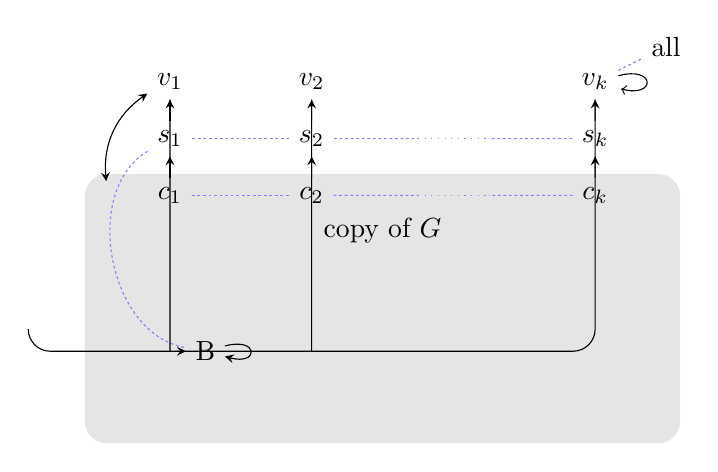
\begin{tikzpicture}[scale=0.9]
                    \draw[copyofG] (-0.2,\ybase-0.3) rectangle (8.2,3.5);
                    \draw (1.5,\ybase) node (nb) {B};
                    \draw (1,4) node (s1) {$s_1$};
                    \draw (3,4) node (s2) {$s_2$};
                    \draw (7,4) node (sk) {$s_k$};
                    \draw (1,3.2) node (t1) {$c_1$};
                    \draw (3,3.2) node (t2) {$c_2$};
                    \draw (7,3.2) node (tk) {$c_k$};
                    \draw (1,4.8) node (v1) {$v_1$};
                    \draw (3,4.8) node (v2) {$v_2$};
                    \draw (7,4.8) node (vk) {$v_k$};
                    \draw (8,5.3) node (all) {all};
                    \draw[-stealth] (t1) -- (s1);
                    \draw[-stealth] (t2) -- (s2);
                    \draw[-stealth] (tk) -- (sk);
                    \draw[tobehere,communication] (s1) -- (s2);
                    \draw[tobehere,communication] (s2) -- (4.5,4);
                    \draw[dotted,color=blue!50!white] (4.5,4) -- (5.5,4);
                    \draw[tobehere,communication] (sk) -- (5.5,4);
                    \draw[tobehere,communication] (t1) -- (t2);
                    \draw[tobehere,communication] (t2) -- (4.5,3.2);
                    \draw[dotted,color=blue!50!white] (4.5,3.2) -- (5.5,3.2);
                    \draw[tobehere,communication] (tk) -- (5.5,3.2);
                    \path[tobehere,communication] (s1) edge[bend right=70] (nb);
                    %\addCommunicationB{s1}
                    \draw[-stealth] (s1) -- (v1);
                    \draw[-stealth] (s2) -- (v2);
                    \draw[-stealth] (sk) -- (vk);
                    \draw[stealth-stealth] (v1) to[bend right] (0.1,3.4);
                    \path (vk) edge [loop right] (vk);
                    \draw[-stealth] (nb) to [loop right] (nb);
                    \draw [-stealth, rounded corners = 8pt] (vk) -- (7,\ymax) -- (-1,\ymax) -- (-1, \ybase)  -- (nb);
                    \draw (v1) -- (1,\ymax);
                    \draw (v2) -- (3,\ymax);
                    \draw[tobehere,communication] (vk) -- (all);
                    \node at (4, 2.7) {copy of $G$};
                \end{tikzpicture}
            }
            \caption{Topological graph $G'$ constructed from the \pbReachDir-instance.}
            \label{figure:topologicgraphproblemcoverage}
        \end{center}
    \end{figure}
    Node $s_1$ can communicate with the base $B$, and node $v_k$ can communicate
    with all nodes of $G'$. Furthermore, we have the communication edges
    $(s_i,s_{i+1})$ and~$(v_i,v_{i+1})$ for all~$1\leq i\leq k-1$.
    Now we prove that the $k$ agents can progress to the
    configuration ($c_1,\dots,c_k$) in $G$  if and only if there exists a
    covering execution in~$G'$.

    ($\Rightarrow$) If the agents are in the configuration ($c_1,\dots,c_k$)
    then they can progress in one step to configuration ($s_1,\dots,s_k$). Then,
    they have no choice but progress to the configuration ($v_1,\dots,v_k$).
    Once in this configuration, the agent placed on the node $v_k$
    communicates with the base and with all other agents. %with any agent, placed on any node, and to the base $B$.
    This agent stays at $v_k$. Meanwhile the agent placed on the
    node $v_1$ will visit all unvisited nodes of $G$ and come back to $v_1$
    while keeping communication to the base through the agent placed on $v_k$.
    Meanwhile, agents placed on $v_2,\dots,v_{k-1}$ come back to $B$. Finally,
    when all the nodes have been visited, both agents on $v_1$ and $v_k$ come
    back to $B$.

    \newcommand{\timesk}{t_{s_k}}

    ($\Leftarrow$) If there exists a covering execution of the whole graph $G'$,
    it means all nodes have been visited. In particular, node $s_k$ has been
    visited and let us consider the first time $\timesk$ when $s_k$ is visited.
    Time $\timesk-1$ denotes the time just before $\timesk$.


    \begin{fact} \label{fact:nodesoutsideGprimeunvisited}
      At time $\timesk-1$, no node $v_i$ and no node~$s_i$ were visited.
    \end{fact}

    \begin{proof}
        Suppose by contradiction that a node $v_i$ was visited by some agent
        before $\timesk$, then the only possibility such an agent to communicate
        to the base is that there is also an agent at $v_k$ at time $\timesk$.
        But then, it means that $s_k$ was visited strictly before $\timesk$,
        leading to a contradiction. Thus, no node $v_i$ were visited at time
        $\timesk$ (thus at time $\timesk-1$).

        As no node $v_i$ are visited before $\timesk$, no node $s_i$ are visited
        before $\timesk-1$.
    \end{proof}


    \begin{fact} \label{fact:reachc1ck}
        At time $\timesk-1$, the configuration is $\langle c_1, \dots, c_k\rangle$.
    \end{fact}

    \begin{proof}
        At time $\timesk$, as the agent at $s_k$ needs to communicate with the base,
        the only
        possibility is that the configuration is $\langle s_1, \dots, s_k\rangle$. Thus, the
        only possibility is that configuration is $\langle c_1, \dots, c_k\rangle$.
    \end{proof}

    Facts~\ref{fact:nodesoutsideGprimeunvisited} implies that the prefix from
    time 0 to time $\timesk-1$ of the covering execution is an execution in $G$.
    Fact~\ref{fact:reachc1ck} implies that sub-execution reaches $\langle
    c_1,\dots,c_k\rangle$.
\end{proof}


% By Proposition~\ref{prop:dir:ub:cover-reach} and Theorem~\ref{th:dir:lb:cover}:

% \begin{theorem} \label{th:dir:compl:cover}
%     \pbCoverageDir is PSPACE-complete.
% \end{theorem}
% \begin{theorem}
%     \label{th:dir:compl:cover}
%   \pbCoverageDir is PSPACE-complete.
% \end{theorem}

%%% Local Variables:
%%% mode: latex
%%% TeX-master: "main"
%%% End:


\section{Neighbor-Communicable Topological Graphs}
\label{sec:nc}

In this subsection, we show that our problems remain hard
for neighbor-communicable graphs.

%The \pbReach{} on the neighbor-communicable topological graphs was proven
%to be PSPACE-complete in \cite{dblp:conf/aaai/tateobrab18}. 
%\todo{Ocan: Removed ref to Tateo}
%We study the \pbCoverage{}problem for this subclass.

\begin{theorem} 
  \label{thm:nc:lb:cover}
  \pbCoverageNC is PSPACE-complete.
\end{theorem}

\begin{proof}
  The upper bound is given by Theorem~\ref{prop:dir:ub:cover-reach}.

  For the lower bound on \pbCoverageNC, the reduction given in
  Figure~\ref{figure:topologicgraphproblemcoverage} is not adapted 
  for neighbor communicable graphs.
  Indeed, all nodes may be visited  although $c_1, \dots, c_k$
  is not reached: $v_1$ and $v_k$ can be reached by two lines of agents
  connected to the base, making the coverage of the full graph possible.
  We nevertheless give a similar reduction by adapting the previous reduction.
  \iffull

  \begin{figure}[t]
        \begin{center}
            \newcommand{\xretourgauche}{-1}
            \tikzstyle{circlenode} =  [circle, draw=black, fill=black, inner sep=0.8mm]
            \newcommand{\ligne}[1]{
            \node[circlenode]  (s1) at (0,#1)  {};
            \node[circlenode]  (s1) at (0.3,#1)  {};
            \node[circlenode]  (s1) at (1,#1)  {};
            \node[circlenode] (s2) at (3,#1)   {};
            \node[circlenode]  (sk) at (7,#1)  {};
            \draw[-stealth] (1, #1-0.5) -- (s1);
            \draw[-stealth] (3, #1-0.5) -- (s2);
            \draw[-stealth] (7, #1-0.5) -- (sk);
            \draw[tobehere,communication] (s1) -- (s2);
            \draw[tobehere,communication] (s2) -- (4.5,#1);
            \draw[dotted,color=green] (4.5,#1) -- (5.5,#1);
            \draw[tobehere,communication] (sk) -- (5.5,#1);}

            \newcommand{\lignevdots}[1]{
            \node[]  (s1) at (1,#1)  {$\vdots$};
            \node[] (s2) at (3,#1)   {$\vdots$};
            \node[]  (sk) at (7,#1)  {$\vdots$};
            \draw[-stealth] (1, #1-0.7) -- (s1);
            \draw[-stealth] (3, #1-0.7) -- (s2);
            \draw[-stealth] (7, #1-0.7) -- (sk);
            }

            \newcommand{\vnodeY}{8.7}
            \newcommand{\posBaseY}{2.75}
            \scalebox{1}
            {
                \begin{tikzpicture}[xscale=0.75,yscale=0.9]
                \draw[copyofG] (-0.2,\posBaseY-0.3) rectangle (8.2,4);
%                \draw (4,\posBaseY	) node[draw] (nb) {B};
                \draw (4,\posBaseY) node (nb) {B};
                \draw (1,3.75) node (t1) {$c_1$};
                \draw (3,3.75) node (t2) {$c_2$};
                \draw (7,3.75) node (tk) {$c_k$};

                \draw[tobehere,communication] (t1) -- (t2);
                \draw[tobehere,communication] (t2) -- (4.5,3.75);
                \draw[dotted,color=green] (4.5,3.75) -- (5.5,3.75);
                \draw[tobehere,communication] (tk) -- (5.5,3.75);


                \ligne {4.5}
                \addCommunicationB {s1}
                \lignevdots {5.25}
                \ligne {5.9}
                \addCommunicationB {s1}

                \node at (7.5, 5.8) {$s_k$};

                \draw[decoration={brace,mirror,raise=5pt},decorate]
                (8,4.3) -- node[right=10pt] {$k+1$} (8, 6);



                \ligne {6.5}
                \addCommunicationB {sk}
                %			\ligne {10.5}
                %			\addCommunicationB {sk}
                \lignevdots {7.25}
                \ligne {7.9}
                \addCommunicationB {sk}


                \draw[decoration={brace,mirror,raise=5pt},decorate]
                (8,6.3) -- node[right=10pt] {$k+1$} (8,8);



                \draw (1,\vnodeY) node (v1) {$v_1$};
                \draw (3,\vnodeY) node (v2) {$v_2$};
                \draw (7,\vnodeY) node (vk) {$v_k$};
                \draw (8,\vnodeY+0.5) node (all) {all};
                \draw[-stealth] (s1) -- (v1);
                \draw[-stealth] (s2) -- (v2);
                \draw[-stealth] (sk) -- (vk);
                \draw[-stealth, rounded corners = 8pt] (v1) -- (0.3, \vnodeY-0.3) -- (0.3,4);
                \draw[stealth-, rounded corners = 8pt] (v1) -- (0, \vnodeY) -- (0,4);

                \path (vk) edge [loop right] (vk);
                \draw[-stealth] (nb) to [loop right] (nb);
                \draw [-stealth, rounded corners = 8pt] (vk) -- (7,\vnodeY+0.5) -- (\xretourgauche,\vnodeY+0.5) -- (\xretourgauche, \posBaseY)  -- (nb);
                \draw (v1) -- (1,\vnodeY+0.5);
                \draw (v2) -- (3,\vnodeY+0.5);

                \draw[tobehere,communication] (vk) -- (all);
                \node at (4, 3.25) {copy of $G$};
                \end{tikzpicture}
            }
            \caption{Topological graph of the \pbCoverageNC-instance constructed from the \pbReachNC-instance for the case of neighbor-communicable topological graph.}
            \label{figure:topologicgraphproblemcoveragefixedforneighborcommunicable}
        \end{center}
    \end{figure}
  
  
	The corrected construction is given in Figure
	\ref{figure:topologicgraphproblemcoveragefixedforneighborcommunicable}. When
	configuration $\langle c_1,...,c_k\rangle$ is reached, the agents go through
	a first layer of length $k+1$ in which the first agent can communicate with
	$B$. Then they go through another layer of length $k+1$ in which the
	$k^{th}$ agent can communicate with $B$. This way, it is mandatory that all
	agents move at the same time to visit $\langle v_1,\dots,v_k\rangle$. Once
	the $k^{th}$ agent is at $v_k$, all agents can communicate with $B$ wherever
	they are, so they can visit remaining states in the copy of $G$. Now let us
	prove that $\langle c_1, \dots, c_k\rangle$ is reachable in $G$ iff it is
	possible to cover all nodes in $G'$.
	
	
	($\Rightarrow$) If $\langle c_1, \dots, c_k\rangle$ is reachable in $G$,
	then we extend the execution to reach $\langle v_1, \dots, v_k\rangle)$ and
	by the same trick as in Figure \ref{figure:topologicgraphproblemcoverage},
	the agent that reaches $v_1$ visits all the remaining unvisited nodes in
	$G$. Thus, we extend the execution for covering all nodes in $G'$.
	
	$(\Leftarrow)$ Suppose all nodes are visited in $G'$. In particular, $v_1$
	and $v_k$ are visited. Let us consider the first moment $t_{v_i}$ when a
	node $v_i$ is visited.
	
	\begin{fact} \label{fact:nodesv1vk}
		At the first moment, the configuration of the agents is $\langle v_1,
		\dots, v_k\rangle$.
	\end{fact}
	
	\begin{proof}
		Let us prove that there is an agent at $v_k$. Suppose that at that
		moment there is no agent at $v_k$. Due to the topological graph $G'$, the
		agent at $v_i$ is disconnected from the base since  nodes that
		communicate directly to $B$ are too far from $v_i$: indeed, the top
		$k+1$-grid is too long and, for $i=1$, the path on left between $v_1$
		and the copy of $G$ is too long. Contradiction.
		
		The agent at $v_k$ came from the unique $2k+2$-long path from $c_k$ to
		$v_k$. Actually, $k+1$ steps before - let us call this moment $t_{s_k}$,
		she was on $s_k$. But at that time, due to the topological graph, there
		are $k$ agents on the row containing $s_k$, otherwise the agent at $s_k$
		would have been disconnected from the base (the bottom $k+1$-grid is too
		long).
		
		So $k+1$ times later $t_{s_k}$, all the $k$ agents are at $\langle v_1,
		\dots, v_k\rangle$.
	\end{proof}
	
	Taking Fact \ref{fact:nodesv1vk} as granted, we consider time $t$ that is
	$2k+2$ steps before and we clearly have the following fact.
	
	\begin{fact}
		At time $t$, the configuration is $\langle c_1, \dots, c_k\rangle$.
	\end{fact}

	Moreover, the following fact holds.
	
	\begin{fact}
		At time $t$, no node outside $G$ were visited.
	\end{fact}
	
	\begin{proof}
		By contradiction, if some node outside $G$ were visited, it means that
		some agent went out the copy of $G$. By definition of $G'$, it would
		mean that a node $v_i$ would have been visited, before time $t$, hence
		strictly before $t_{v_i}$. Contradiction.
	\end{proof}

	To sum up, the prefix of the execution from $\langle B, \dots, B\rangle$ to
	$\langle c_1, \dots, c_k\rangle$ is fully inside the copy of $G$. So
  $\langle c_1, \dots, c_k\rangle$ is reachable in $G$.
  
  \else

  The details are given in the long version.

  \fi

\end{proof}

%By Proposition~\ref{prop:nc:lb:cover} and


% \begin{theorem}
% \label{th:nc:compl:cover}
% \pbCoverageNC is PSPACE-complete.
% \end{theorem}

%%% Local Variables:
%%% mode: latex
%%% TeX-master: "main"
%%% End:


\section{Sight-Moveable Topological Graphs}
\label{sec:sm}

%\textbf{\textcolor{red}{Proofs density 5.1-5.4}}

In this subsection, we show that \pbReachSM and \pbCoverageSM
are in LOGSPACE while the bounded version \pbBReachSM is
NP-complete.

\subsection{Upper bounds}

The results in this subsection are based on a result of Reingold~\cite{Reingold:2008}, who
proved that the problem of checking the connectivity of two nodes $s$ and $t$ in an
undirected graph, namely \USTCONN, is in LOGSPACE.

\begin{theorem}
	\label{theorem:USTCONNinLOGSPACE}
	\USTCONN~ is in LOGSPACE \cite{Reingold:2008}.
\end{theorem}

\begin{proposition}\label{prop:sm:ub:reach}
	\pbReachSM is in LOGSPACE.
\end{proposition}

\begin{proof}
  The idea of the proof is to reduce \pbReachSM to \UCONN, that is the problem
  of deciding whether an undirected graph is connected. From
  Theorem~\ref{theorem:USTCONNinLOGSPACE}, we can reduce \UCONN~ to \USTCONN~
  by simply looping over all pairs of nodes ($\sourcenode, \targetnode)$ and
  checking for a path from $\sourcenode$ to $\targetnode$. Therefore, \UCONN~
  is in LOGSPACE.

  Now we describe the logarithmic space reduction of \pbReachSM
  \linebreak[4]
  to \UCONN. Let $G=\langle \setnodes, \moves, \coms \rangle$ a sight-moveable
    topological graph and $c$ a configuration. Let $\setnodes' = \set{c_1,
    \dots, c_n, \basenode}$. The configuration $c$ is reachable iff the
    restriction of $\myundirectedgraph := (\setnodes, \coms)$ to the nodes in
    $\setnodes'$ is $\coms$-connected. Indeed, if it is, then $c$ is reachable:
    each agent follows some $\moves$-path from $\basenode$ to $c_i$ contained in
    a $\coms$-path from $\basenode$ to $c_i$. In other words, $(G, c)$ is a
    positive \pbReachSM-instance iff $\myundirectedgraph$ is a positive
    \UCONN-instance. The reduction is in logarithmic space: we compute
    $\myundirectedgraph$ by enumerating all $(u, v)$ $\coms$-edges in $G$, and
    we output $(u, v)$ when $u, v \in \setnodes'$. We recall that we only take
    into account the working memory for computing $\myundirectedgraph$; the
    output -- $\myundirectedgraph$ itself -- is not taken into account in the
    used space (see e.g. \cite{DBLP:books/daglib/0086373}, Ch. 8, Def. 8.21).
\end{proof}



%We denote $Comm(S)=\{v \in V / \exists u \in S, v \coms u\}$ the set of nodes
%which communicates with a node in $S$.
%We obtain that the algorithm \pbReachSM is sound and complete for the problem
%of reachability of a configuration in a topological graph. The \pbReachSM
%problem is then in P given that the algorithm \pbReachSM computes the fixed
%point on $S$ in polynomial-time.

% \end{comment}


\begin{proposition}\label{prop:sm:ub:cover}
  \pbCoverageSM is in LOGSPACE.
\end{proposition}

\begin{proof}
  First we prove that the bounded version of the connectivity in undirected
  graphs is also in LOGSPACE.

  \begin{lemma}
    \label{lemma:boundedUSTCONNinLOGSPACE}
    Bounded-\USTCONN, that is the problem, giving an undirected graph
    $\myundirectedgraphbounded$, two nodes $\sourcenode, \targetnode$, an
    integer $n$ written in binary, of deciding whether there is a path of
    length at most $n$ from $\sourcenode$ to $\targetnode$ in $G$ is in
    LOGSPACE.
  \end{lemma}

  \begin{proof} We reduce Bounded-\USTCONN~ to \USTCONN~ in logarithmic space as
    follows. From a Bounded-\USTCONN~ instance $(\myundirectedgraphbounded,
    \sourcenode, \targetnode, n)$ we construct in logarithmic space a
    \USTCONN~ instance $(\myundirectedgraph, \sourcenode', \targetnode')$:
    \begin{inparaenum}
    \item The nodes of $\myundirectedgraph$ are pairs $(v, j)$ where $v$
      is a node of $\myundirectedgraphbounded$ and $j$ is an integer in
      $\set{0,n}$ but smaller than the number of nodes in
      $\myundirectedgraph$;
    \item $\myundirectedgraph$ contains an edge between $(v, j)$ and
      $(v', j+1)$ when there is an edge between $v$ and $v'$ in
      $\myundirectedgraphbounded$ or when $v = v'$;
    \item $\sourcenode' = (\sourcenode, 0)$ and $\targetnode' =
      (\targetnode', n)$.
    \end{inparaenum}
  \end{proof}

  Now let $G=\langle V, \moves, \coms \rangle$ be a sight-moveable topologic
  graph and $n$ an integer written in binary. To test whether $(G, n)$ is a
  positive instance of Coverage, it suffices to check that there is a path
  from any node $v$ to the base $B$ with at most $n$ communication edges. To
  do that, we test sequentially, for all $v$, that $((V, \coms), v, B, n)$ is
  a positive instance of Bounded-\USTCONN~. Thus, we obtain an algorithm in
  logarithmic space to decide Coverage.

\end{proof}

%%% Local Variables:
%%% mode: latex
%%% TeX-master: "main"
%%% End:


\subsection{Lower bounds}


We now focus on the NP lower bound of \pbBReachSM. 
% We
% recall the 3-satisfiability (3-SAT) problem which is
% NP-complete~\cite{DBLP:conf/coco/Karp72}.

% \begin{definition}[3-SAT] The 3-satisfiability problem is the following decision
%   problem:
%   \begin{itemize}
%   \item[] Input: a set of $n$ variables $\booleanvariablegeneric_1, \dots,
%     \booleanvariablegeneric_n$ and a set of $m$ disjunctive clauses
%     $\clausegeneric_1, \dots, \clausegeneric_m$. Each clause contains up to 3
%     literals (a variable or its negation).
% %  \item[] Output: does there exists an assignment for the variables satisfying
% %  all clauses ?
%   \item[] Output: is there a variable assignment satisfying all clauses?
% %does there exists an assignment for the variables satisfying
% %  all clauses ?
%   \end{itemize}
% \end{definition}

% \begin{theorem}
%   3-SAT problem is NP-complete \cite{DBLP:conf/coco/Karp72}.
% \end{theorem}

\iffull
\begin{figure*}
    \begin{center}
    \vspace{1cm}
    \scalebox{0.75}{
    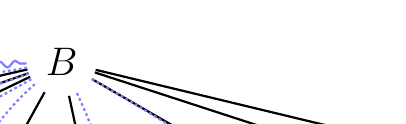
\begin{tikzpicture}[node distance=2cm,thick,
      main node/.style={font=\sffamily\Large\bfseries,minimum size=0.5cm},
      staging node/.style={circle,fill=black}]
  
      \node[main node,circle] (B) {$\basenode$};
      \draw[use as bounding box] (B.center)+(4cm,0);
      \node (VAR) [below left=0cm and 2cm of B] {};
      \node (VAR1) [left=4cm of VAR] {};
      \node (VAR3) [right=4cm of VAR] {};
  
      \node[staging node] (SX1) [below left of=VAR1] {};
      \node[main node] (X1) [below of=SX1] {$\booleanvariablegeneric_1$};
      \node[staging node] (SNX1) [below right of=VAR1] {};
      \node[main node] (NX1) [below of=SNX1] {$\neg \booleanvariablegeneric_1$};
      \node[main node] (GX1) [below right of=SX1] {$g_{\booleanvariablegeneric_1}$};
  
      \node[staging node] (SX2) [below left of=VAR] {};
      \node[main node] (X2) [below of=SX2] {$\booleanvariablegeneric_2$};
      \node[staging node] (SNX2) [below right of=VAR] {};
      \node[main node] (NX2) [below of=SNX2] {$\neg \booleanvariablegeneric_2$};
      \node[main node] (GX2) [below right of=SX2] {$g_{\booleanvariablegeneric_2}$};
  
      \node[staging node] (SX3) [below left of=VAR3] {};
      \node[main node] (X3) [below of=SX3] {$\booleanvariablegeneric_3$};
      \node[staging node] (SNX3) [below right of=VAR3] {};
      \node[main node] (NX3) [below of=SNX3] {$\neg \booleanvariablegeneric_3$};
      \node[main node] (GX3) [below right of=SX3] {$g_{\booleanvariablegeneric_3}$};
  
      \node[staging node] (P3) [below of=GX1] {};
      \node[staging node] (P2) [left=2cm of P3] {};
      \node[staging node] (P1) [left=2cm of VAR1] {};
  
      \node (CLA) [below right=0cm and 3cm of B] {};
      \node (CLA1) [right=2cm of CLA] {};
      \node (CLA2) [right=4cm of CLA] {};
      
      \node[staging node] (SC1) [below=1.1cm of CLA1] {};
      \node[main node] (C1) [below of=SC1] {$\clausegeneric_1$};
      \node[main node] (GC1) [below of=C1] {$g_{\clausegeneric_1}$};
  
      \node[staging node] (SC2) [below=1.1cm of CLA2] {};
      \node[main node] (C2) [below of=SC2] {$\clausegeneric_2$};
      \node[main node] (GC2) [below of=C2] {$g_{\clausegeneric_2}$};
      
      \foreach \i in {1,...,3}{\path (B) edge (SX\i);}
      \foreach \i in {1,...,3}{\path (B) edge (SNX\i);}
      \foreach \i in {1,...,3}{\path (SX\i) edge (X\i);}
      \foreach \i in {1,...,3}{\path (SNX\i) edge (NX\i);}
      \foreach \i in {1,...,3}{\path (X\i) edge (GX\i);}
      \foreach \i in {1,...,3}{\path (NX\i) edge (GX\i);}
  
      \foreach \i in {1,...,2}{\path (B) edge (SC\i);}
      \foreach \i in {1,...,2}{\path (SC\i) edge (C\i);}
      \foreach \i in {1,...,2}{\path (C\i) edge (GC\i);}
  
      \path[communication,tobehere]
      (B) edge [out=190, in=90] (X1)
      edge [out=200, in=90] (NX1)
      edge [out=210, in=90] (X2)
      edge [bend right=35] (NX2)
      edge [bend left=20] (X3)
      edge [out=330, in=90] (NX3)
      % edge [out=337, in=90] (C1)
      % edge [out=345, in=90] (C2)
      ;
      \path
      (GX1) edge [bend right=60] (GX2)
      (GX2) edge [bend right=60] (GX3)
      (GX3) edge (GC1)
      (GC1) edge (GC2);
      \draw[tobehere,decorate,decoration={snake,amplitude=.4mm,segment length=2mm}] (GX1) -- (P3);
      \draw[tobehere,decorate,decoration={snake,amplitude=.4mm,segment length=2mm}] (P3) -- (P2);
      \draw[tobehere,decorate,decoration={snake,amplitude=.4mm,segment length=2mm}] (P2) -- (P1);
      \draw[tobehere,decorate,decoration={snake,amplitude=.4mm,segment length=2mm}] (P1) -- (B);
      %(GC2) edge [bend right] (CLA2)
      %(CLA2) edge [bend right] (B)
      %(CLA2) edge [bend right] (CLA2.center)
      %(CLA2) edge [bend left] (CLA2.center)
      
      \path
  
      (C1) edge [bend left, blue!50!red](X1)
      edge [bend left, blue!50!red] (NX2)
      edge [bend left, blue!50!red] (X3)
  
      (C2) edge [bend left, red!50!white] (X2)
      edge [bend left, red!50!white] (X3)
      
      ;
    \end{tikzpicture}
    }
    
    % \vspace{4.2cm}
    % \vspace{5cm}
    \hspace{13.2cm}		
    \raisebox{-1.5cm}{
      \fbox{
        \tiny
        \begin{tabular}{ll}
          \tikz{\draw (0, 0) edge (0.4, 0);} & Movement \\
          \tikz{\draw[communication, tobehere] (0, 0) edge (0.4, 0);} & Communication \\
          \tikz{\draw[tobehere,decorate,decoration={snake,amplitude=.4mm,segment
          length=2mm}] (0, 0) -- (0.4, 0);} & Fully connected \\
          \tikz{\draw[blue!50!red] (0, 0) edge (0.4, 0);} & \multirow{2}{*}{Clauses dependencies}\\
          \tikz{\draw[red!50!white] (0, 0) edge (0.4, 0);} &
        \end{tabular}
        }
    }
    \end{center}
    \vspace{1.8cm}
    \caption{Graph construction from the formula $(x_1 \vee \neg x_2 \vee x_3) \wedge (x_2 \vee x_3)$.}
    \label{fig:cons}
  \end{figure*}

  \begin{figure}
    \centering
    \begin{subfigure}{.23\textwidth}
      \centering
      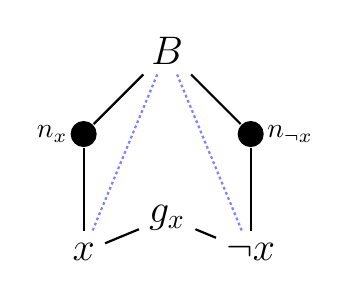
\begin{tikzpicture}[node distance=1.5cm,
                      thick,
                      main node/.style={,font=\sffamily\Large\bfseries,minimum size=0.5cm},
                      staging node/.style={circle,fill=black}]
  
        \node[main node] (1) {$\basenode$};
        \node[staging node] (2) [below left of=1]{};
        \node[left of=2, node distance=0.4cm] {$n_x$};
        \node[main node] (3) [below of=2] {$\booleanvariablegeneric$};
        \node[staging node] (4) [below right of=1] {};
        \node[right of=4, node distance=0.5cm] {$n_{\lnot x}$};
        \node[main node] (5) [below of=4] {$\neg \booleanvariablegeneric$};
  
        \node[main node] (6) [below right of=2] {$g_\booleanvariablegeneric$};
  
        \path[every node/.style={font=\sffamily\small}]
        (1) edge (2)
        (2) edge (3)
        (3) edge (6)
  
        (1) edge (4)
        (4) edge (5)
        (5) edge (6)
        ;
  
        \path[communication,tobehere]
        (1) edge (3)
        (1) edge (5)
        ;
    \end{tikzpicture}
    \caption{Variable gadget.}
    \label{fig:Gvar}
    \end{subfigure}%
    \begin{subfigure}{.23\textwidth}
      \centering
      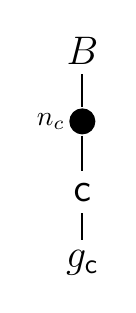
\begin{tikzpicture}[node distance=0.9cm,
                      thick,
                      main node/.style={font=\sffamily\Large\bfseries,minimum size=0.5cm},
                      staging node/.style={circle,fill=black}]
  
        \node[main node] (1) {$\basenode$};
        \node[staging node] (2) [below of=1] {};
        \node[left of=2,node distance=0.4cm] {$n_c$};
        \node[main node] (3) [below of=2] {$\clausegeneric$};
        \node[main node] (4) [below of=3] {$g_\clausegeneric$};
  
        \path[every node/.style={font=\sffamily\small}]
        (1) edge (2)
        (2) edge (3)
        (3) edge (4)
        ;
  
        % \path[dashed,tobehere]
        % (1) edge [bend right] (3)
        % ;
    \end{tikzpicture}
    \caption{Clause gadget.}
    \label{fig:Gcla}
    \end{subfigure}
    \caption{Translation gadgets}
  \end{figure}
\else
\input{picture_sight_small}
\fi

\begin{proposition} \label{prop:sm:lb:breach}
  \pbBReachSM is NP-hard for a fixed execution length $\ell\geq 3$.
\end{proposition}
\begin{proof}
  The proof is by polynomial time reduction from 3-SAT problem (see \cite{DBLP:conf/coco/Karp72}).
  Given a 3-SAT instance, set of clauses $c_1,\ldots,c_m$ with variables~$x_1,\ldots,x_n$,
  we describe the
  construction of an instance $(G, c)$ of \pbBReachSM \linebreak with~$k=n+m$ agents.
%  \todo{Possible confusion between~$c$ and~$c_1,\ldots,c_m$}


% We construct the graph $G=\langle V,E,C\rangle$ from an instance of 3-SAT.
%The topological graph contains a node for each literal, a goal node for each variable, a node and a goal node for each clause. Then, a clause exactly communicates with the literal it is
  %associated with. In order to reach a clause, an agent must be placed at one of
 % the literals of the former to preserve communication.
  %
  The topological graph $G=\langle\setnodes, \moves, \coms \rangle$ is constructed
  as follows. We start by placing the base $\basenode$ from which the agents start
  their mission.

  Please recall that a sight-moveable graph is also a neighbor-communicable graph so
  all movements edges are also communication edges in the construction below
  even if not explicitly stated.

  For each variable $\booleanvariablegeneric$, we construct a gadget composed of
  5 nodes connected to the base depicted in Figure \ref{fig:Gvar}:  nodes
  $\booleanvariablegeneric$, $\neg \booleanvariablegeneric$, staging nodes
  $n_\booleanvariablegeneric$, $n_{\neg \booleanvariablegeneric}$ and a
  \emph{goal} node $g_\booleanvariablegeneric$. We add movement edges from $B$
  to $n_\booleanvariablegeneric$, from $n_\booleanvariablegeneric$ to
  $\booleanvariablegeneric$ and from $\booleanvariablegeneric$ to
  $g_\booleanvariablegeneric$ (resp. from $B$ to $n_{\neg
  \booleanvariablegeneric}$, from $n_{\neg \booleanvariablegeneric}$ to $\neg
  \booleanvariablegeneric$ and from $\neg \booleanvariablegeneric$ to
  $g_\booleanvariablegeneric$). As for the communication, the node
  $\booleanvariablegeneric$ (res. $\neg \booleanvariablegeneric$) communicates
  with the base. %The staging nodes are not labeled in the figures for clarity.

  For each clause $\clausegeneric$, we construct a gadget composed of 3
  nodes depicted in Figure \ref{fig:Gcla}. We create a node $\clausegeneric$, a
  staging node $n_\clausegeneric$ and a goal node $g_\clausegeneric$. We add
  movement edges from $B$ to $n_c$, from $n_\clausegeneric$ to $\clausegeneric$
  and from $\clausegeneric$ to $g_\clausegeneric$. 
  %As in the variable gadget,
  %the node $\clausegeneric$ communicates with the base. 
  The communication between a clause $\clausegeneric$ and a literal
  $\booleanvariablegeneric$ or $\neg \booleanvariablegeneric$ is dictated by the
  existence of the literal in the clause: $\clausegeneric_i\coms
  \booleanvariablegeneric_j$ if and only if~$\booleanvariablegeneric_j \in
  \clausegeneric_i$; and $\clausegeneric_i\coms \lnot \booleanvariablegeneric_j$
  if and only if~$\lnot \booleanvariablegeneric_j \in \clausegeneric_i$.

  We add movement edges from
  $g_{\booleanvariablegeneric_i}$ to $g_{\booleanvariablegeneric_{i+1}}$,
  and from $g_{\clausegeneric_i}$ to~$g_{\clausegeneric_{i+1}}$ for all~$1 \leq i < n$,
  as well as we from
   $g_{\booleanvariablegeneric_n}$ to $g_{\clausegeneric_1}$.
   Last, we add a fully connected path containing 3 fresh nodes from $g_{\booleanvariablegeneric_1}$ to the base such that $g_{\booleanvariablegeneric_1} \coms \basenode$,
   in the sense that all nodes of this path have communication edges between them.
  This translation is polynomial in the number of clauses and variables.
  The construction is depicted in Figure~\ref{fig:cons}.
  The snake-like path from $g_{\booleanvariablegeneric_1}$ to $\basenode$ is the
  fully connected path.

  From a 3-SAT instance, one can construct the graph $G$ and ask for an
  execution of length 3 to reach the configuration \linebreak $\langle
  g_{\booleanvariablegeneric_1}, \dots, g_{\booleanvariablegeneric_n},
  g_{\clausegeneric_1}, \dots, g_{\clausegeneric_m}\rangle$.


  \iffull
  \begin{fact}
    $G$ is a sight-moveable topological graph.
  \end{fact}
  \begin{proof}
    One can see that the single communication edges created by the construction,
    apart from the ones induced by the movement, are the communication between
    the base $B$ and the nodes $\booleanvariablegeneric_i$ and $\neg
    \booleanvariablegeneric_i$. Hence, a path does exist under the communication
    of $B$ to reach $\booleanvariablegeneric_i$.
  \end{proof}

  Now let us prove that a 3-SAT instance is satisfiable iff there exists an
  execution of at most 3 steps in the graph $G$.

  ($\Rightarrow$) We show that if a 3-SAT instance is satisfiable then there
  exists an execution of at most 3 steps in the graph $G$ built from it. Let
  $val$ be a truth assignment which satisfies the instance.
  Recall that there are~$n+m$ agents.
  The first step of the execution consists in moving an agent in each~$n_{c_i}$,
  and for each variable~$x_j$, moving one agent to~$n_{x_j}$ if the $val(x_j)=1$
  and to~$n_{\lnot x_j}$ otherwise.
  Note that all staging nodes communicate with~$\basenode$ since the graph
  is neighbor-communicable.

  In the second step, all agents progress to their unique successors other than~$\basenode$.
  While all nodes~$x_j$ and~$\lnot x_j$ are connected to~$\basenode$,
  a node~$c_i$ is connected to~$\basenode$ if and only if there is an
  agent in one of its literals. This is the case since $val$ satisfies the formula.
  In the third step of the execution, agents go to states~$g_{x_j}$ and~$g_{c_i}$.
  Here, the connection with the base is ensured since~$g_{x_1}$ is connected
  to it, and~$g_{x_2}$ is connected to~$g_{x_1}$, $g_{x_3}$ is connected to~$g_{x_2}$ and
  so on.

  This execution is thus a solution of \pbBReachSM with bound $\ell=3$.

  ($\Leftarrow$) We now show that if there exists an execution of at most 3
  steps in the graph $G$ constructed from a 3-SAT instance, then the instance is
  satisfiable. Assume we have an execution $e$ of at most 3 steps with the last
  configuration being $\langle g_{\booleanvariablegeneric_1}, \dots,
  g_{\booleanvariablegeneric_n}, g_{\clausegeneric_1}, \dots,
  g_{\clausegeneric_m}\rangle$.

  The only shortest path from $\basenode$ to~$g_{c_i}$ is of length~$3$ and goes through
  $n_{c_i}$. For states $g_{x_j}$, the only shortest paths are also of length~$3$
  and go through either $n_{x_j}$ or~$n_{\lnot x_j}$. Thus, in order to reach the given
  target configuration, at the initial step, agents must cover the states~$n_{c_i}$
  and either~$n_{x_j}$ or~$n_{\lnot x_j}$ for all $i,j$. At the second step,
  following the above mentioned shortest paths, agents will be at states~$c_i$
  and either~$x_j$ or~$\lnot x_j$ depending on the staging nodes they were occupying.
  The last step is the target configuration.
  Since the agents are connected at the second, it follows that for each clause~$c_i$,
  the state corresponding to some literal of~$c_i$ is occupied by an agent.
  Thus the valuation on variables encoded by the choices of the agents satisfies the
  3-SAT instance.

  \else
  The rest of the proof is given in the long version.
  \fi
  % First, given the length of the execution, one
  % can observe that for each variable $\booleanvariablegeneric_i$ only the node
  % $\booleanvariablegeneric_i$ or $\neg \booleanvariablegeneric_i$ has been
  % visited, with $0<i\leq n$. Second, the $m$ agents in the clause nodes
  % $g_\clausegeneric$ required an agent to be located at one of the variable
  % nodes connected to it. Given that a clause is only connected to its literals,
  % an agent can access a clause iff another is placed at a node which satisfies
  % it.
\end{proof}

From Propositions~\ref{prop:dir:ub:bcover-breach} and~\ref{prop:sm:lb:breach}, we have:

\begin{theorem} \label{th:sm:compl:breach}
  \pbBReachSM is NP-complete.
\end{theorem}

%%% Local Variables:
%%% mode: latex
%%% TeX-master: "main"
%%% End:


\section{Complete-Communication Topological Graphs}
\label{sec:compl}

%In this section, we show that \pbBReachCC is in LOGSPACE and that \pbBCoverageCC
%is NP-complete.

%\subsection{Upper bounds}

The following result relies on the fact that the communication constraints are
trivial this class.

\begin{proposition}
    \label{prop:cc:ub:breach}
    \pbBReachCC is in LOGSPACE.
\end{proposition}
\begin{proof}
    From Lemma \ref{lemma:boundedUSTCONNinLOGSPACE}, one can construct an
    algorithm in LOGSPACE for \pbBReachCC. Indeed, given a configuration $c$ and
    $\ell\in\mathds{N}$, the straightforward iteration on the locations $c_i$
    followed by the verification of a path of at most $\ell$ (given in unary) steps from
    $\basenode$ to $c_i$ yields a sound and complete algorithm for \pbBReachCC.
\end{proof}


%\subsection{Lower bounds}

Our NP lower bound proof of the \pbBCoverageCC problem is by reduction from
the grid Hamiltonian cycle (G-HC) problem which is the Hamiltonian cycle problem
restricted to grid graphs and is NP-complete~\cite{Itai:1982}.
%\todo{What is a grid graph?}

% \begin{definition}[G-HC] The grid Hamiltonian cycle problem is the following
%   decision problem:
% %  \begin{itemize}
% %  \item[] Input:
%   Given a grid graph $G=\langle V,E \rangle$,
% %  \item[] Output:
%     decide if there is a simple cycle $t$ in $G$ which contains all vertices?
%     %such that
%     %all $v\in V$ are seen only once in $t$?
% %    does there exist a tour $t$ in $G$, that is a path such that
% %    all $v\in V$ are seen only once in $t$?
%   \end{itemize}
% \end{definition}

%\begin{theorem}
%  G-HC problem is NP-complete \cite{Itai:1982}.
%\end{theorem}
%Our result is by reduction from G-HC:
\begin{theorem} \label{prop:cc:lb:bcover}
  \label{th:cc:compl:bcover}
  \pbBCoverageCC is NP-complete.
\end{theorem}
\iffull
\begin{proof}
  The upper bound follows from Proposition~\ref{prop:dir:ub:bcover-breach}.
  
  We give a polynomial-time reduction from the G-HC problem.
  Consider a graph~$G=\langle V, E\rangle$, an instance of~G-HC.
  %We describe
  %the construction of an instance of \pbBCoverageCC from a G-HC instance below.

  Consider the sight-moveable topological graph %\linebreak[4] 
  $G'=\langle V,
  \moves, \coms\rangle$ with $\moves~=E$ and $\coms=V\times V$ and associate a
  single agent and the bound~$|V|$ to the \pbBCoverageCC instance.
  We call a simple cycle containing all vertices a \emph{tour}.
  We prove that there exists a tour $t$ in $G$ iff there exists a
  covering execution of length $|V|$ in $G'$.

  ($\Rightarrow$) Any tour of~$G$ is a valid execution satisfying
  \pbBCoverageCC since the communication edges form a complete graph,
  and the bound is~$|V|$.

  ($\Leftarrow$) Let us suppose that we have an execution of length $|V|$
  which covers the graph $G'$. The execution starts and ends at $\basenode$
  and
  visits all nodes in $|V|$ steps. Hence, the execution visits all nodes only
  once and is a cycle in the graph.

  
\end{proof}
\else
The upper bound follows from Proposition~\ref{prop:dir:ub:bcover-breach}. The
  NP-hardness proof is given in the long version.
\fi

% \begin{theorem}
%   \label{th:cc:compl:bcover}
%   \pbBCoverageCC is NP-complete.
% \end{theorem}

%%% Local Variables:
%%% mode: latex
%%% TeX-master: "main"
%%% End:


\section{Related Work}
\label{sec:relate}
\iffull
\begin{figure}[!t]
  \centering
  {\footnotesize
      \begin{tabular}{l|c|c|c|c}
        & $Reach$ & $Cover$ & $bReach$ & $bCover$
        \\\hline
        
        Directed & PSPACE-c & PSPACE-c &
        \multirow{3}{*}{\shortstack{NP-c\\ {[Hollinger]}}} &%\nocite{Hollinger:2012}}} &
        \multirow{5}{*}{NP-c} \\
        \cline{1-3}

        NC & \multirow{2}{*}{\shortstack{PSPACE-c\\ {[Tateo et al.]}}} %\nocite{dblp:conf/aaai/tateobrab18}}}
        & PSPACE-c & &
        % \\
        % \begin{tikzpicture}
        %   \node (s) at (0, 0) {};
        %   \node (t) at (3, 0) {};
        %   \draw[->] (s) -- (t);
        %   \draw[communication,tobehere] (s) edge[bend right=20] (t);
        % \end{tikzpicture} & & & & 
        \\
        % &&&&\\
        \cline{1-1}\cline{3-3}


        Undirected & & ? & & % \\  
        % \begin{tikzpicture}
        %   \node (s) at (0, 0) {};
        %   \node (t) at (3, 0) {};
        %   \draw[-] (s) -- (t);
        %   \draw[communication,tobehere] (s) edge[bend right=20] (t);
        % \end{tikzpicture} & & & &
        \\\cline{1-4}
        
        SM &
        \multirow{2}{*}{in L} &
        \multirow{2}{*}{in L} &
        NP-c &
        % \\ 
        % \begin{tikzpicture}
        %   \node (s) at (0, 0) {};
        %   \node (t) at (3, 0) {};
        %   \node (1) at (1, -0.5) {};
        %   \node (2) at (2, -0.5) {};
        %   \draw[communication] (s) -- (t);
        %   \draw[-, tobehere] (s) -- (1);
        %   \draw[-, tobehere] (1) -- (2);
        %   \draw[-, tobehere] (2) -- (t);
        %   \draw[communication, tobehere] (s) edge[bend right=10] (1);
        %   \draw[communication, tobehere] (1) edge[bend right=10] (2);
        %   \draw[communication, tobehere] (2) edge[bend right=10] (t);
        %   \draw[communication, tobehere] (1) edge[bend right=4] (t);
        %   \draw[communication, tobehere] (s) edge[bend right=4] (2);
        % \end{tikzpicture} & & &$(k=3)$  &
        \\
        \cline{1-1}\cline{4-4}

        
        CM & & &
        in L & \\
        % \\
        %  \begin{tikzpicture}
        %  \node (1) at (0.5, 0) {};
        %  \node (2) at (2.5, 0) {};
        %  \node (3) at (1, -0.5) {};
        %  \node (4) at (2, -0.5) {};
        %  \node (5) at (1.5, 0.5) {};
        %  \foreach \x in {1, ..., 5} {
        %  \foreach \y in {1, ..., 5} {
        %  	\draw[communication,tobehere] (\x) -- (\y);
        %  }}
        %  \end{tikzpicture} & & &  & ($d=1$) \\ 
      \end{tabular}
  }
  \caption{Complexity results.}
  \label{fig:results}
\end{figure}
\else
\begin{figure}[!t]
  \centering
  {\footnotesize
      \begin{tabular}{l|c|c|c|c}
        & $Reach$ & $Cover$ & $bReach$ & $bCover$
        \\\hline
        
        Directed & PSPACE-c & PSPACE-c &
        \multirow{3}{*}{\shortstack{NP-c\\ {[Hollinger]}}} &%\nocite{Hollinger:2012}}} &
        \multirow{5}{*}{NP-c} \\
        \cline{1-3}

        NC & \multirow{2}{*}{\shortstack{PSPACE-c\\ {[Tateo et al.]}}} %\nocite{dblp:conf/aaai/tateobrab18}}}
        & PSPACE-c & &
        % \\
        % \begin{tikzpicture}
        %   \node (s) at (0, 0) {};
        %   \node (t) at (3, 0) {};
        %   \draw[->] (s) -- (t);
        %   \draw[communication,tobehere] (s) edge[bend right=20] (t);
        % \end{tikzpicture} & & & & 
        \\
        % &&&&\\
        \cline{1-1}\cline{3-3}


        Undirected & & ? & & % \\  
        % \begin{tikzpicture}
        %   \node (s) at (0, 0) {};
        %   \node (t) at (3, 0) {};
        %   \draw[-] (s) -- (t);
        %   \draw[communication,tobehere] (s) edge[bend right=20] (t);
        % \end{tikzpicture} & & & &
        \\\cline{1-4}
        
        SM &
        \multirow{2}{*}{in L} &
        \multirow{2}{*}{in L} &
        NP-c &
        % \\ 
        % \begin{tikzpicture}
        %   \node (s) at (0, 0) {};
        %   \node (t) at (3, 0) {};
        %   \node (1) at (1, -0.5) {};
        %   \node (2) at (2, -0.5) {};
        %   \draw[communication] (s) -- (t);
        %   \draw[-, tobehere] (s) -- (1);
        %   \draw[-, tobehere] (1) -- (2);
        %   \draw[-, tobehere] (2) -- (t);
        %   \draw[communication, tobehere] (s) edge[bend right=10] (1);
        %   \draw[communication, tobehere] (1) edge[bend right=10] (2);
        %   \draw[communication, tobehere] (2) edge[bend right=10] (t);
        %   \draw[communication, tobehere] (1) edge[bend right=4] (t);
        %   \draw[communication, tobehere] (s) edge[bend right=4] (2);
        % \end{tikzpicture} & & &$(k=3)$  &
        \\
        \cline{1-1}\cline{4-4}

        
        CM & & &
        in L & \\
        % \\
        %  \begin{tikzpicture}
        %  \node (1) at (0.5, 0) {};
        %  \node (2) at (2.5, 0) {};
        %  \node (3) at (1, -0.5) {};
        %  \node (4) at (2, -0.5) {};
        %  \node (5) at (1.5, 0.5) {};
        %  \foreach \x in {1, ..., 5} {
        %  \foreach \y in {1, ..., 5} {
        %  	\draw[communication,tobehere] (\x) -- (\y);
        %  }}
        %  \end{tikzpicture} & & &  & ($d=1$) \\ 
      \end{tabular}
  }
  \caption{Complexity results.}
  \label{fig:results}
\end{figure}
\fi
The coverage planning is an interesting approach to path planning. Indeed, a
covering plan can be used for fields such as floor cleaning, lawn mowing, etc. A
survey of this field appears in \cite{Choset:01}. This multi-agent extension has
the ability to reduce the length of the overall mission and also reach parts of
the area a single agent would not able to. This problem was studied in
\cite{Rekleitis:97} for two agents. As shown in the survey by Chen et al.
\cite{ChenSurvey}, many coverage problems have been addressed by using analytic
techniques. For instance, in \cite{DBLP:conf/icc/Yanmaz12} and
\cite{teacy2010maintaining}, they consider UAVs that should cover an area
while staying connected to the base, but only empirically study some path planning
algorithms without proving their algorithms formally.
%planning algorithms and their algorithms are not proven formally but only
%tested experimentally.

We advocate formal methods that give formal guarantees and have already been applied to
generate plans for robots and UAVs. Model checking has been
applied to robot planning (see \cite{DBLP:conf/iros/LacerdaPH14}) and to UAVs~\cite{webster2011formal}.
Humphrey \cite{Humphrey2013} shows how to use LTL (linear-temporal logic) model
checking for capturing response and fairness properties in cooperation (for
instance, if a task is requested then it is eventually performed). 
%Model
%checking has also been used to verify pre-programmed UAVs
%\cite{webster2011formal}.

% In \cite{DBLP:journals/corr/abs-1003-0381}, they discuss CTL model checking
% for checking properties. CTL is not suitable for our purpose because we need
% to express the existence of \emph{one} path along which UAVs stay connected
% and eventually have covered all the locations and have come back to the base
% location.

Bodin et al. \cite{IJCAI2018demodrones} treat a similar problem except that the
UAVs cover the graph without returning to the base. Without the return-to-the-base
constraint, we claim that all our hardness results still hold, except
for \pbBCoverageCC. They provide an implementation by describing the problem in
Planning Domain Description Language and then run the planner
Functional Strips \cite{DBLP:conf/ijcai/FrancesRLG17}.

% Both \pbReach{} and \pbCoverage{} may be expressed in MA-STRIPS
% \cite{DBLP:conf/aips/BrafmanD08}, that is a multi-agent variant of STRIPS
% (Stanford Research Institute Problem Solver) in which actions for each agent
% can be described independently. The representation in multi-agent planning
% languages is especially efficient when actions of the different agents are
% independent and when they required to coordinate not so often. However, as the
% agents should maintain connection, it requires a lot of coordination.

Murano et al. \cite{DBLP:conf/prima/MuranoPR15} advocate for a
graph-theoretic representations of states, that is, by assigning locations to
agents as in Definition~\ref{def:config}. In
\cite{DBLP:conf/atal/AminofMRZ16,DBLP:conf/atal/Rubin15}, a general formalism is given to specify LTL and monadic second-order logic properties,
which are expressive enough to describe the connectivity constraint.
%Indeed, linear temporal operators enable to express that any vertex
%should be visited in the future and the connectivity invariant. MSO on the
%topological graph enables to express the connectivity as a fix point (the
%subgraph made up of the UAVs and the base is connected).
They provide an
algorithm for parametrized verification in the sense that they check a temporal
property in a class of graphs. This is relevant for partially-known
environments. The algorithm described is
non-elementary %\footnote{\todo[inline]{explain non-elementary}}
(\textit{i.e.} the running time cannot bounded by any tower of exponentials)
and therefore not
usable in practice. We believe that this is an important problem
and our paper identifies an efficient and relevant fragment.
%studying fragments of this is
%relevant, and our paper identifies a relevant fragment.

The multiple traveling salesman problem (mTSP) is a generalization of the
traveling salesman problem (TSP) in which multiple salesmen are located at a
depot \cite{Anbuudayasankar:2016}. mTSP asks for the coverage of all cities so as to minimize the total plan cost by visiting each city exactly once.
%This generalization of TSP is considered as a
%relaxation of the vehicle routing problem (VRP) in which the capacity constraint
%is removed.
An overview of TSP and its extensions are presented
\cite{Matai:2010}. The \pbCoverage{} problem is related to mTSP, since we use
results on Hamiltonian cycle to prove the NP-hardness of \pbBCoverageCC.
However, we wish to minimize the length of the execution and not the cost of the
execution. Those problems are equivalent on unit graphs, but it is not trivial
to use general results on mTSP in order to solve \pbCoverage{}. Furthermore, to
the best of our knowledge, connected versions of mTSP and VRP have not been
studied.

%%% Local Variables:
%%% mode: latex
%%% TeX-master: "main"
%%% End:



\section{Conclusion}
\label{sec:concl}
% In this work, we extended the study of multi agent connected path planning 
% by considering the coverage problem. We showed that in the general case the complexity of the
% decision of the coverage matches the complexity of the reachability problem.
% Furthermore, this complexity still holds for the neighbor-communicable
% subclass.
% We identified an important subclass of topological graphs on which the complexity
% of the problem is as low as LOGSPACE.
% Unfortunately, the bounded
% versions of both problems stays NP-complete.
% A LOGSPACE algorithm can be obtained by ignoring communication constraints,
% that is, for the complete-communication subclass.
%However, an even more restrictive
%subclass admits a logarithmic-space algorithm for the bounded reachability
%problem.

%We can observe that the
Sight-moveable topological graphs we introduced in this work only constrain
the communication graph. One can be interested to constrain the movement graph
to a planar graph or a 2D grid given the common usage of grid modelling of the
environment. Given the intractability of MAPP on planar graphs \cite{Yu:2015}
and on general 2D grid graphs \cite{Banfi:2017}, it is likely that this
problem is intractable as well. Furthermore, in
\cite{dblp:conf/aaai/tateobrab18}, the decision is proved to stay
PSPACE-complete on planar graphs and grids as well. However, one can study this
problem on solid grid graphs, given that the Hamiltonian cycle is tractable on
such graphs \cite{Umans:1997}.

One can note that our NP lower bound reductions hold without the
anonymity of the agents. Indeed, the \pbBCoverage{} case is straightforward and for \pbBReach{} case, each agent can be associated to a clause or variable, so the reduction would still hold.
%Thus, the lower bound holds without anonymity.
%\todo{Ocan: Do we claim in the sense of conjecture or do we state it? Please avoid using claim in the latter sense}

We do not know  if \pbCoverage{} remains hard when the
$\rightarrow$-relations become symmetric, depicted in Figure~\ref{fig:results}
as a question mark. We think this open issue is important since symmetric
{$\rightarrow$-relations} (if UAVs can go from $v$ to $v'$, they can also come
back from $v'$ to $v$) are relevant for practical applications. We plan to
study the \emph{parametrized complexity} \cite{DBLP:series/mcs/DowneyF99} of our
problems - parameters could be the treewidth of the topological graph, the
number of UAVs.

% \todo{Can we remove following two paragraphs?}
% We attend to develop efficient parallel algorithms for the problems proven in
% LOGSPACE. Those algorithms can yield feasible solution in a short amount of time
% in order to be improved by heuristic-based algorithms. The sight-moveable
% topological graphs being a ``simpler'' class than the undirected ones, we can
% hope to obtain a polynomial-time approximation algorithm. Furthermore, this
% class seems to admit an intuitive resolution process which involve finding the
% relay positions and optimizing the coverage of multiple small areas.

% Interestingly, we plan to generalize to decentralized versions of our problems
% and to dynamic environments. Instead of generating sequences of actions, we will
% have to generate strategies as in ATL (alternating-time temporal logic)
% \cite{DBLP:journals/corr/abs-1006-1414}. As UAVs stay connected, we may suppose
% that when information is gained, it is common knowledge and that all actions,
% especially sensing actions, are public \cite{DBLP:conf/atal/BelardinelliLMR17}.
% We also aim at using a high-level dedicated formal logic to express objectives,
% such as the language proposed in \cite{DBLP:conf/atal/Rubin15} and
% \cite{DBLP:conf/atal/AminofMRZ16}.

%%% Local Variables:
%%% mode: latex
%%% TeX-master: "main"
%%% End:


%%% Local Variables:
%%% mode: latex
%%% TeX-master: "main"
%%% End:


\appendix

\bibliographystyle{named}
\bibliography{biblio}

\end{document}


%%%%%%%%%%%%%%%%%%%%%%%%%%%%%


%% your usepackages here:
% \usepackage{times}  %Required
% \usepackage{helvet}  %Required
% \usepackage{courier}  %Required
% \usepackage{url}  %Required
% \usepackage{graphicx}  %Required
% \usepackage{soul}
% \usepackage[utf8]{inputenc}
% \usepackage[usenames, dvipsnames]{xcolor}
% \usepackage{amsmath}
% \usepackage{amsthm}

% \usepackage{subfig}



%% do not change the following lines
% \setcopyright{ifaamas}  % do not change this line!
% \acmDOI{doi}  % do not change this line!
% \acmISBN{}  % do not change this line!
% \acmConference[AAMAS'19]{Proc.\@ of the 18th International Conference on Autonomous Agents and Multiagent Systems (AAMAS 2019), N.~Agmon, M.~E.~Taylor, E.~Elkind, M.~Veloso (eds.)}{May 2019}{Montreal, Canada}  % do not change this line!
% \acmYear{2019}  % do not change this line!
% \copyrightyear{2019}  % do not change this line!
% \acmPrice{}  % do not change this line!







% DO NOT COMMIT UNCOMMENTED
% \pagecolor[rgb]{0.1,0.1,0.1} \color[rgb]{0.9,0.9,0.9}
%

%%%%%%%%%%%%%%%%%%%%%%%%%%%%%%%%%%%%%%%%%%%%%%%%%%%%%%%%%%%%%%%%%%%%%%%%%%%%%%%%%%%%%%%%%%%%%%%%%%%%%%%%%

% \begin{document}


%\titlenote{Produces the permission block, and copyright information}

% AAMAS: as appropriate, uncomment one subtitle line; check the CFP
%\subtitle{Extended Abstract}
%\subtitle{Industrial Applications Track}
%\subtitle{Socially Interactive Agents Track}
%\subtitle{Blue Sky Ideas Track}
%\subtitle{Engineering Multiagent Systems Track}
%\subtitle{Robotics Track}
%\subtitle{JAAMAS Track}
%\subtitle{Doctoral Mentoring Program}

%\subtitlenote{The full version of the author's guide is available as \texttt{acmart.pdf} document}


% AAMAS: submissions are anonymous for most tracks
% \author{Paper \#185}  % put your paper number here!

%% example of author block for camera ready version of accepted papers: don't use for anonymous submissions
%
% \author{Tristan Charrier}
% \authornote{None.}
% \orcid{1234-5678-9012}
% \affiliation{%
% 	\institution{Univ Rennes, CNRS}
% 	\streetaddress{263 Avenue G\'en\'eral Leclerc}
% 	\city{Rennes} 
% 	\postcode{35042}
% }
% \email{tristan.charrier@irisa.fr}
%
% \author{Arthur Queffelec}
% \authornote{None.}
% \affiliation{%
% 	\institution{Univ Rennes, CNRS}
% 	\streetaddress{263 Avenue G\'en\'eral Leclerc}
% 	\city{Rennes} 
% 	\postcode{35042}
% }
% \email{arthur.queffelec@irisa.fr}
%
% \author{Ocan Sankur}
%  \affiliation{%
% 	\institution{Univ Rennes, CNRS}
% 	\streetaddress{263 Avenue G\'en\'eral Leclerc}
% 	\city{Rennes} 
% 	\postcode{35042}
% }
% \email{ocan.sankur@irisa.fr}
%
% \author{Fran\c{c}ois Schwarzentruber}
%  \affiliation{%
% 	\institution{Univ Rennes, CNRS}
% 	\streetaddress{263 Avenue G\'en\'eral Leclerc}
% 	\city{Rennes} 
% 	\postcode{35042}
% }
% \email{francois.schwarzentruber@ens-rennes.fr}
%\renewcommand{\shortauthors}{B. Trovato et al.}


% \keywords{multi-agent systems; path planning; connectivity constraint; theoretical complexity}  % put your semicolon-separated keywords here!



%%%%%%%%%%%%%%%%%%%%%%%%%%%%%%%%%%%%%%%%%%%%%%%%%%%%%%%%%%%%%%%%%%%%%%%%%%%%%%%%%%%%%%%%%%%%%%%%%%%%%%%%%
%% start of main body of paper




%%%%%%%%%%%%%%%%%%%%%%%%%%%%%%%%%%%%%%%%%%%%%%%%%%%%%%%%%%%%%%%%%%%%%%%%%%%%%%%%%%%%%%%%%%%%%%%%%%%%%%%%%
%% bibliography: see CFP for number of permitted pages

% \clearpage

% \bibliographystyle{ACM-Reference-Format}  % do not change this line!
% \bibliography{biblio}  % put name of your .bib file here

% \end{document}

%%% Local Variables:
%%% mode: latex
%%% TeX-master: t
%%% End:
